% Options for packages loaded elsewhere
\PassOptionsToPackage{unicode}{hyperref}
\PassOptionsToPackage{hyphens}{url}
\PassOptionsToPackage{dvipsnames,svgnames,x11names}{xcolor}
%
\documentclass[
  letterpaper,
  DIV=11,
  numbers=noendperiod]{scrartcl}

\usepackage{amsmath,amssymb}
\usepackage{iftex}
\ifPDFTeX
  \usepackage[T1]{fontenc}
  \usepackage[utf8]{inputenc}
  \usepackage{textcomp} % provide euro and other symbols
\else % if luatex or xetex
  \usepackage{unicode-math}
  \defaultfontfeatures{Scale=MatchLowercase}
  \defaultfontfeatures[\rmfamily]{Ligatures=TeX,Scale=1}
\fi
\usepackage{lmodern}
\ifPDFTeX\else  
    % xetex/luatex font selection
\fi
% Use upquote if available, for straight quotes in verbatim environments
\IfFileExists{upquote.sty}{\usepackage{upquote}}{}
\IfFileExists{microtype.sty}{% use microtype if available
  \usepackage[]{microtype}
  \UseMicrotypeSet[protrusion]{basicmath} % disable protrusion for tt fonts
}{}
\makeatletter
\@ifundefined{KOMAClassName}{% if non-KOMA class
  \IfFileExists{parskip.sty}{%
    \usepackage{parskip}
  }{% else
    \setlength{\parindent}{0pt}
    \setlength{\parskip}{6pt plus 2pt minus 1pt}}
}{% if KOMA class
  \KOMAoptions{parskip=half}}
\makeatother
\usepackage{xcolor}
\setlength{\emergencystretch}{3em} % prevent overfull lines
\setcounter{secnumdepth}{-\maxdimen} % remove section numbering
% Make \paragraph and \subparagraph free-standing
\ifx\paragraph\undefined\else
  \let\oldparagraph\paragraph
  \renewcommand{\paragraph}[1]{\oldparagraph{#1}\mbox{}}
\fi
\ifx\subparagraph\undefined\else
  \let\oldsubparagraph\subparagraph
  \renewcommand{\subparagraph}[1]{\oldsubparagraph{#1}\mbox{}}
\fi

\usepackage{color}
\usepackage{fancyvrb}
\newcommand{\VerbBar}{|}
\newcommand{\VERB}{\Verb[commandchars=\\\{\}]}
\DefineVerbatimEnvironment{Highlighting}{Verbatim}{commandchars=\\\{\}}
% Add ',fontsize=\small' for more characters per line
\usepackage{framed}
\definecolor{shadecolor}{RGB}{241,243,245}
\newenvironment{Shaded}{\begin{snugshade}}{\end{snugshade}}
\newcommand{\AlertTok}[1]{\textcolor[rgb]{0.68,0.00,0.00}{#1}}
\newcommand{\AnnotationTok}[1]{\textcolor[rgb]{0.37,0.37,0.37}{#1}}
\newcommand{\AttributeTok}[1]{\textcolor[rgb]{0.40,0.45,0.13}{#1}}
\newcommand{\BaseNTok}[1]{\textcolor[rgb]{0.68,0.00,0.00}{#1}}
\newcommand{\BuiltInTok}[1]{\textcolor[rgb]{0.00,0.23,0.31}{#1}}
\newcommand{\CharTok}[1]{\textcolor[rgb]{0.13,0.47,0.30}{#1}}
\newcommand{\CommentTok}[1]{\textcolor[rgb]{0.37,0.37,0.37}{#1}}
\newcommand{\CommentVarTok}[1]{\textcolor[rgb]{0.37,0.37,0.37}{\textit{#1}}}
\newcommand{\ConstantTok}[1]{\textcolor[rgb]{0.56,0.35,0.01}{#1}}
\newcommand{\ControlFlowTok}[1]{\textcolor[rgb]{0.00,0.23,0.31}{#1}}
\newcommand{\DataTypeTok}[1]{\textcolor[rgb]{0.68,0.00,0.00}{#1}}
\newcommand{\DecValTok}[1]{\textcolor[rgb]{0.68,0.00,0.00}{#1}}
\newcommand{\DocumentationTok}[1]{\textcolor[rgb]{0.37,0.37,0.37}{\textit{#1}}}
\newcommand{\ErrorTok}[1]{\textcolor[rgb]{0.68,0.00,0.00}{#1}}
\newcommand{\ExtensionTok}[1]{\textcolor[rgb]{0.00,0.23,0.31}{#1}}
\newcommand{\FloatTok}[1]{\textcolor[rgb]{0.68,0.00,0.00}{#1}}
\newcommand{\FunctionTok}[1]{\textcolor[rgb]{0.28,0.35,0.67}{#1}}
\newcommand{\ImportTok}[1]{\textcolor[rgb]{0.00,0.46,0.62}{#1}}
\newcommand{\InformationTok}[1]{\textcolor[rgb]{0.37,0.37,0.37}{#1}}
\newcommand{\KeywordTok}[1]{\textcolor[rgb]{0.00,0.23,0.31}{#1}}
\newcommand{\NormalTok}[1]{\textcolor[rgb]{0.00,0.23,0.31}{#1}}
\newcommand{\OperatorTok}[1]{\textcolor[rgb]{0.37,0.37,0.37}{#1}}
\newcommand{\OtherTok}[1]{\textcolor[rgb]{0.00,0.23,0.31}{#1}}
\newcommand{\PreprocessorTok}[1]{\textcolor[rgb]{0.68,0.00,0.00}{#1}}
\newcommand{\RegionMarkerTok}[1]{\textcolor[rgb]{0.00,0.23,0.31}{#1}}
\newcommand{\SpecialCharTok}[1]{\textcolor[rgb]{0.37,0.37,0.37}{#1}}
\newcommand{\SpecialStringTok}[1]{\textcolor[rgb]{0.13,0.47,0.30}{#1}}
\newcommand{\StringTok}[1]{\textcolor[rgb]{0.13,0.47,0.30}{#1}}
\newcommand{\VariableTok}[1]{\textcolor[rgb]{0.07,0.07,0.07}{#1}}
\newcommand{\VerbatimStringTok}[1]{\textcolor[rgb]{0.13,0.47,0.30}{#1}}
\newcommand{\WarningTok}[1]{\textcolor[rgb]{0.37,0.37,0.37}{\textit{#1}}}

\providecommand{\tightlist}{%
  \setlength{\itemsep}{0pt}\setlength{\parskip}{0pt}}\usepackage{longtable,booktabs,array}
\usepackage{calc} % for calculating minipage widths
% Correct order of tables after \paragraph or \subparagraph
\usepackage{etoolbox}
\makeatletter
\patchcmd\longtable{\par}{\if@noskipsec\mbox{}\fi\par}{}{}
\makeatother
% Allow footnotes in longtable head/foot
\IfFileExists{footnotehyper.sty}{\usepackage{footnotehyper}}{\usepackage{footnote}}
\makesavenoteenv{longtable}
\usepackage{graphicx}
\makeatletter
\def\maxwidth{\ifdim\Gin@nat@width>\linewidth\linewidth\else\Gin@nat@width\fi}
\def\maxheight{\ifdim\Gin@nat@height>\textheight\textheight\else\Gin@nat@height\fi}
\makeatother
% Scale images if necessary, so that they will not overflow the page
% margins by default, and it is still possible to overwrite the defaults
% using explicit options in \includegraphics[width, height, ...]{}
\setkeys{Gin}{width=\maxwidth,height=\maxheight,keepaspectratio}
% Set default figure placement to htbp
\makeatletter
\def\fps@figure{htbp}
\makeatother

\KOMAoption{captions}{tableheading}
\makeatletter
\makeatother
\makeatletter
\makeatother
\makeatletter
\@ifpackageloaded{caption}{}{\usepackage{caption}}
\AtBeginDocument{%
\ifdefined\contentsname
  \renewcommand*\contentsname{Table of contents}
\else
  \newcommand\contentsname{Table of contents}
\fi
\ifdefined\listfigurename
  \renewcommand*\listfigurename{List of Figures}
\else
  \newcommand\listfigurename{List of Figures}
\fi
\ifdefined\listtablename
  \renewcommand*\listtablename{List of Tables}
\else
  \newcommand\listtablename{List of Tables}
\fi
\ifdefined\figurename
  \renewcommand*\figurename{Figure}
\else
  \newcommand\figurename{Figure}
\fi
\ifdefined\tablename
  \renewcommand*\tablename{Table}
\else
  \newcommand\tablename{Table}
\fi
}
\@ifpackageloaded{float}{}{\usepackage{float}}
\floatstyle{ruled}
\@ifundefined{c@chapter}{\newfloat{codelisting}{h}{lop}}{\newfloat{codelisting}{h}{lop}[chapter]}
\floatname{codelisting}{Listing}
\newcommand*\listoflistings{\listof{codelisting}{List of Listings}}
\makeatother
\makeatletter
\@ifpackageloaded{caption}{}{\usepackage{caption}}
\@ifpackageloaded{subcaption}{}{\usepackage{subcaption}}
\makeatother
\makeatletter
\@ifpackageloaded{tcolorbox}{}{\usepackage[skins,breakable]{tcolorbox}}
\makeatother
\makeatletter
\@ifundefined{shadecolor}{\definecolor{shadecolor}{rgb}{.97, .97, .97}}
\makeatother
\makeatletter
\makeatother
\makeatletter
\makeatother
\ifLuaTeX
  \usepackage{selnolig}  % disable illegal ligatures
\fi
\IfFileExists{bookmark.sty}{\usepackage{bookmark}}{\usepackage{hyperref}}
\IfFileExists{xurl.sty}{\usepackage{xurl}}{} % add URL line breaks if available
\urlstyle{same} % disable monospaced font for URLs
\hypersetup{
  pdftitle={Extracting schematic information from tabular PDF documents using a large language model pipeline},
  pdfauthor={Jonathan Jayes - Lund University},
  colorlinks=true,
  linkcolor={blue},
  filecolor={Maroon},
  citecolor={Blue},
  urlcolor={Blue},
  pdfcreator={LaTeX via pandoc}}

\title{Extracting schematic information from tabular PDF documents using
a large language model pipeline}
\usepackage{etoolbox}
\makeatletter
\providecommand{\subtitle}[1]{% add subtitle to \maketitle
  \apptocmd{\@title}{\par {\large #1 \par}}{}{}
}
\makeatother
\subtitle{23-01-2024 - Machine Learning in Economic History Workshop}
\author{Jonathan Jayes - Lund University}
\date{}

\begin{document}
\maketitle
\ifdefined\Shaded\renewenvironment{Shaded}{\begin{tcolorbox}[interior hidden, enhanced, boxrule=0pt, borderline west={3pt}{0pt}{shadecolor}, sharp corners, frame hidden, breakable]}{\end{tcolorbox}}\fi

\hypertarget{sec-motivation}{%
\section{Motivation}\label{sec-motivation}}

What do we as economic historians love?

\begin{figure}

{\centering 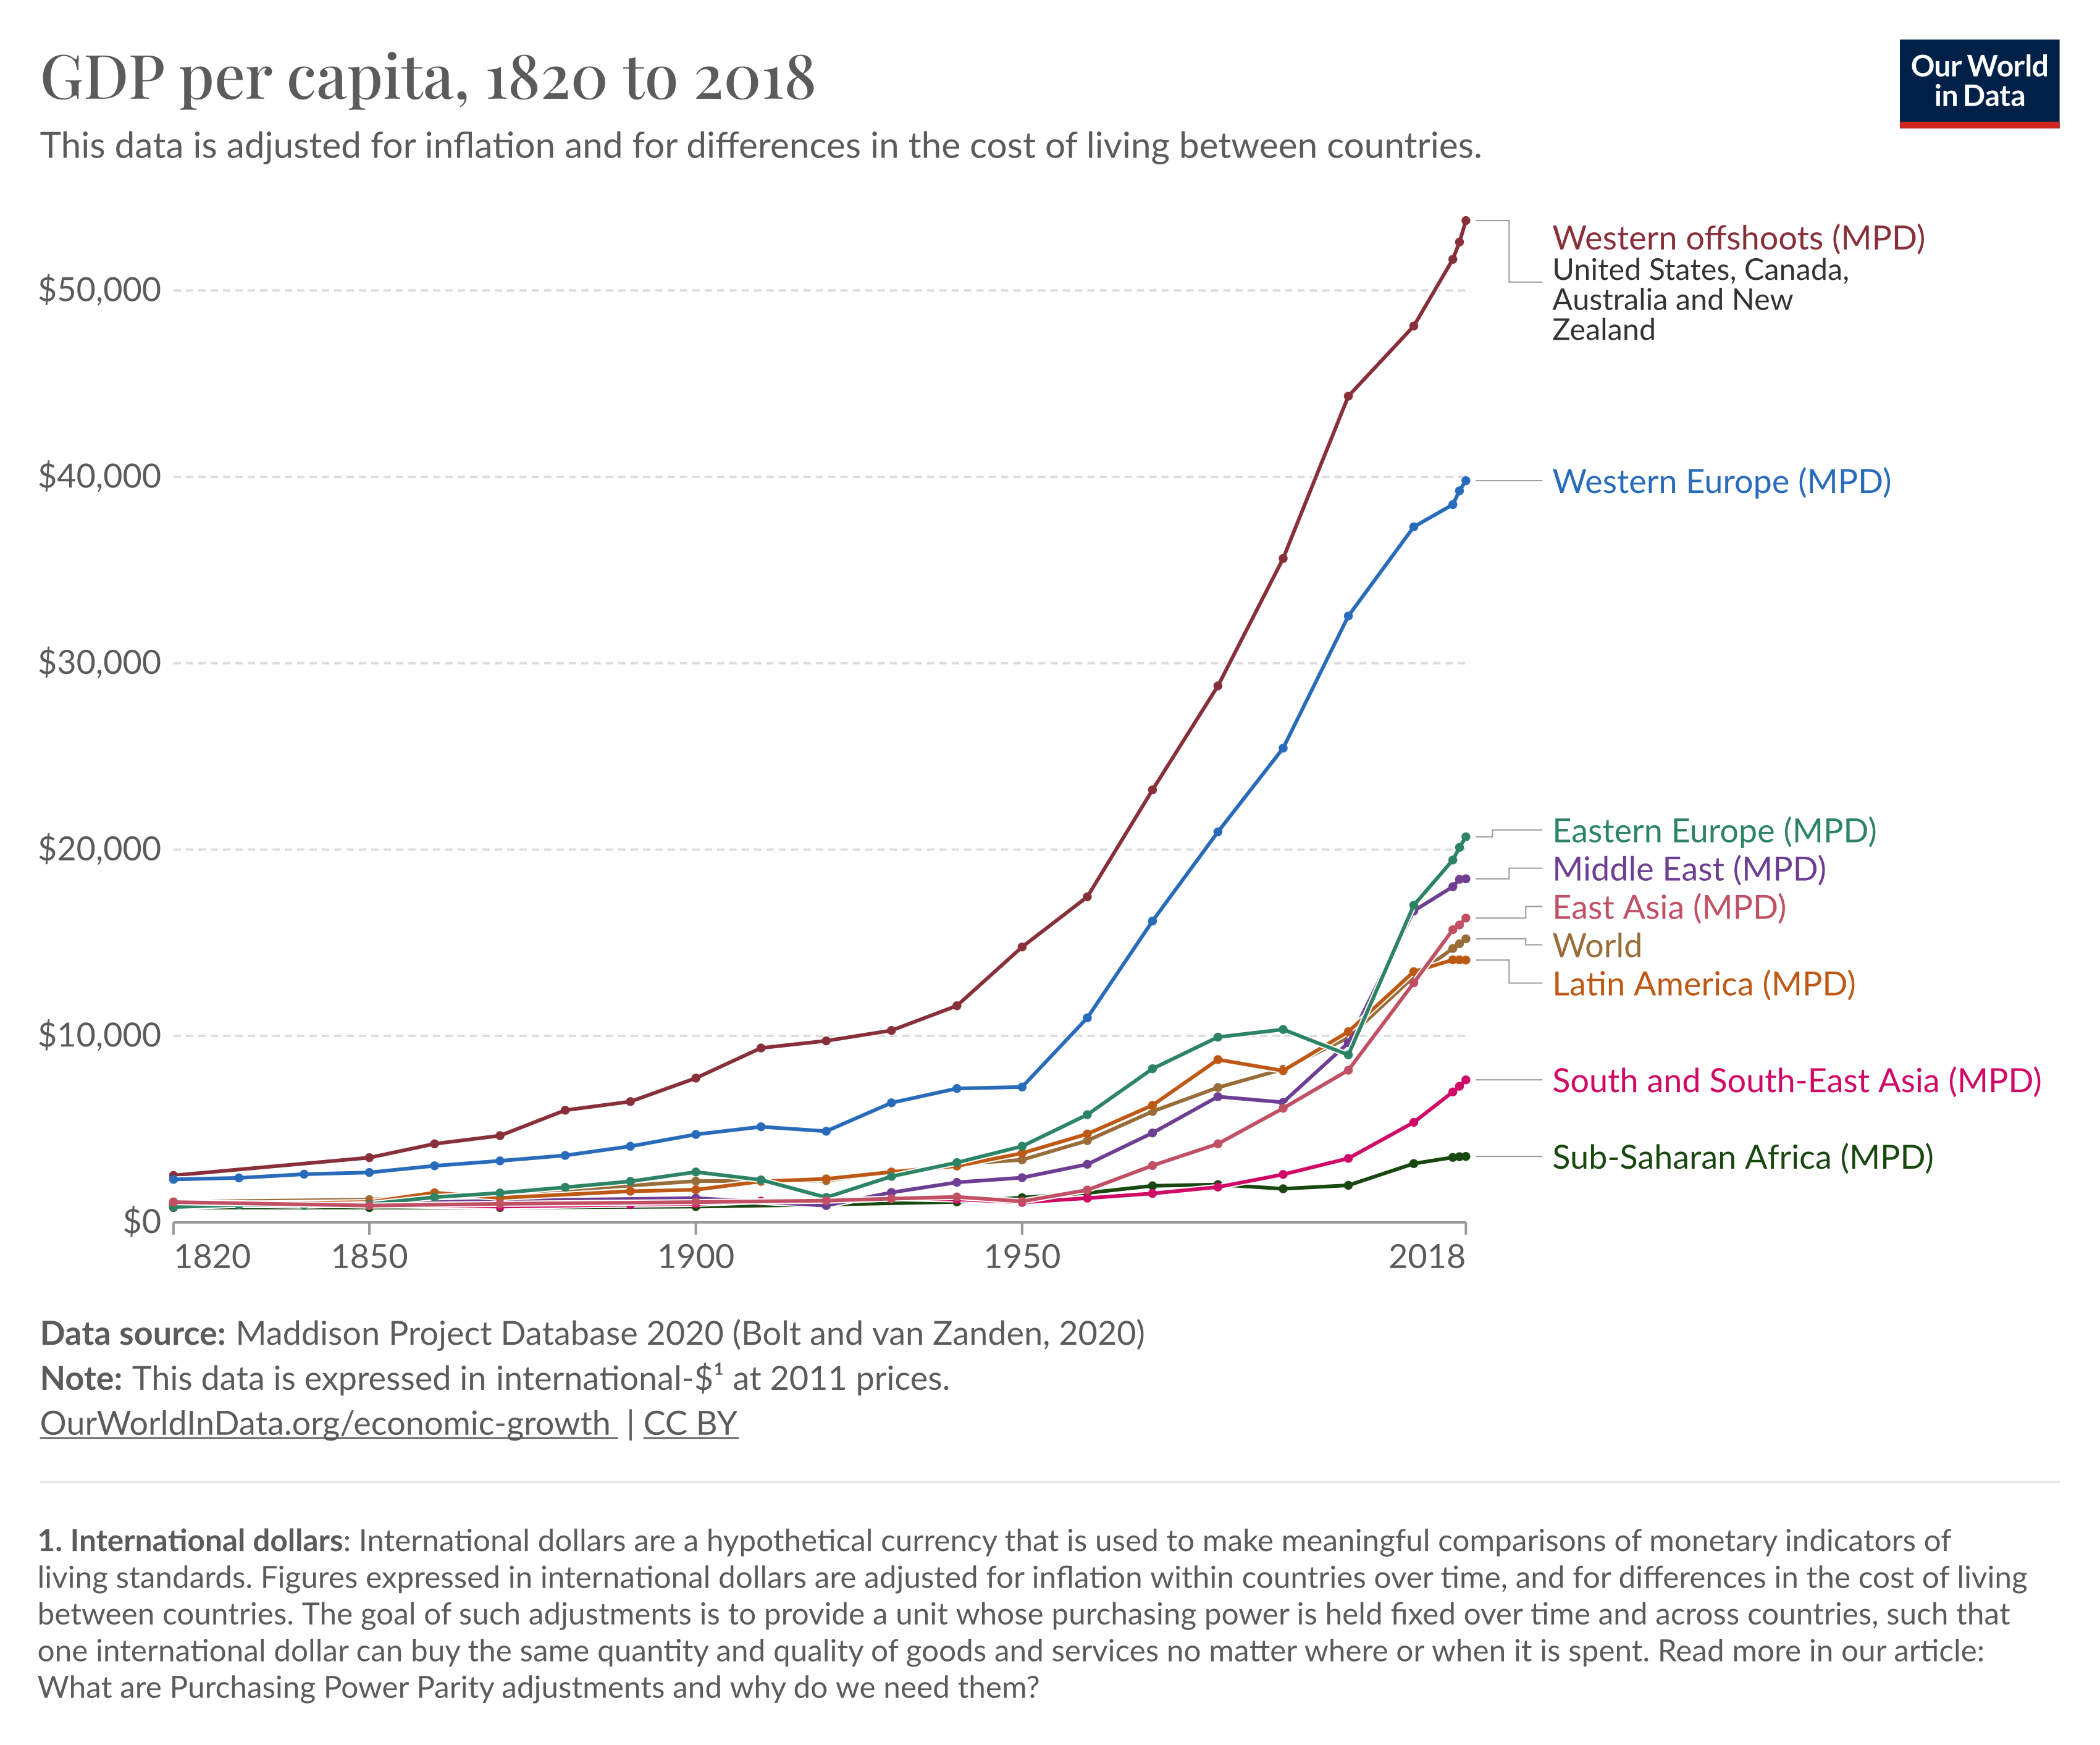
\includegraphics{assets/gdp-per-capita-maddison.png}

}

\caption{Lovely long time series}

\end{figure}

What do we hate?

\begin{figure}

{\centering 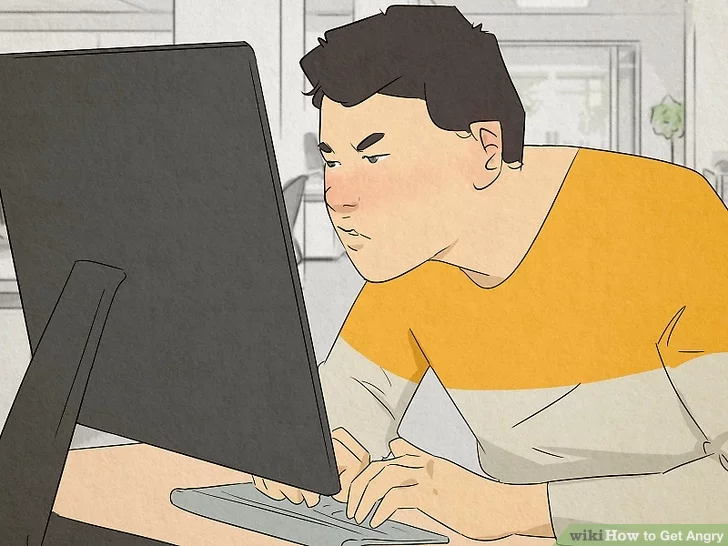
\includegraphics{assets/wikihow.jpeg}

}

\caption{Lots of time spent typing things into excel}

\end{figure}

\hypertarget{what-is-possible-with-off-the-shelf-ocr-tech}{%
\subsection{What is possible with off-the-shelf OCR
tech?}\label{what-is-possible-with-off-the-shelf-ocr-tech}}

\begin{figure}

{\centering 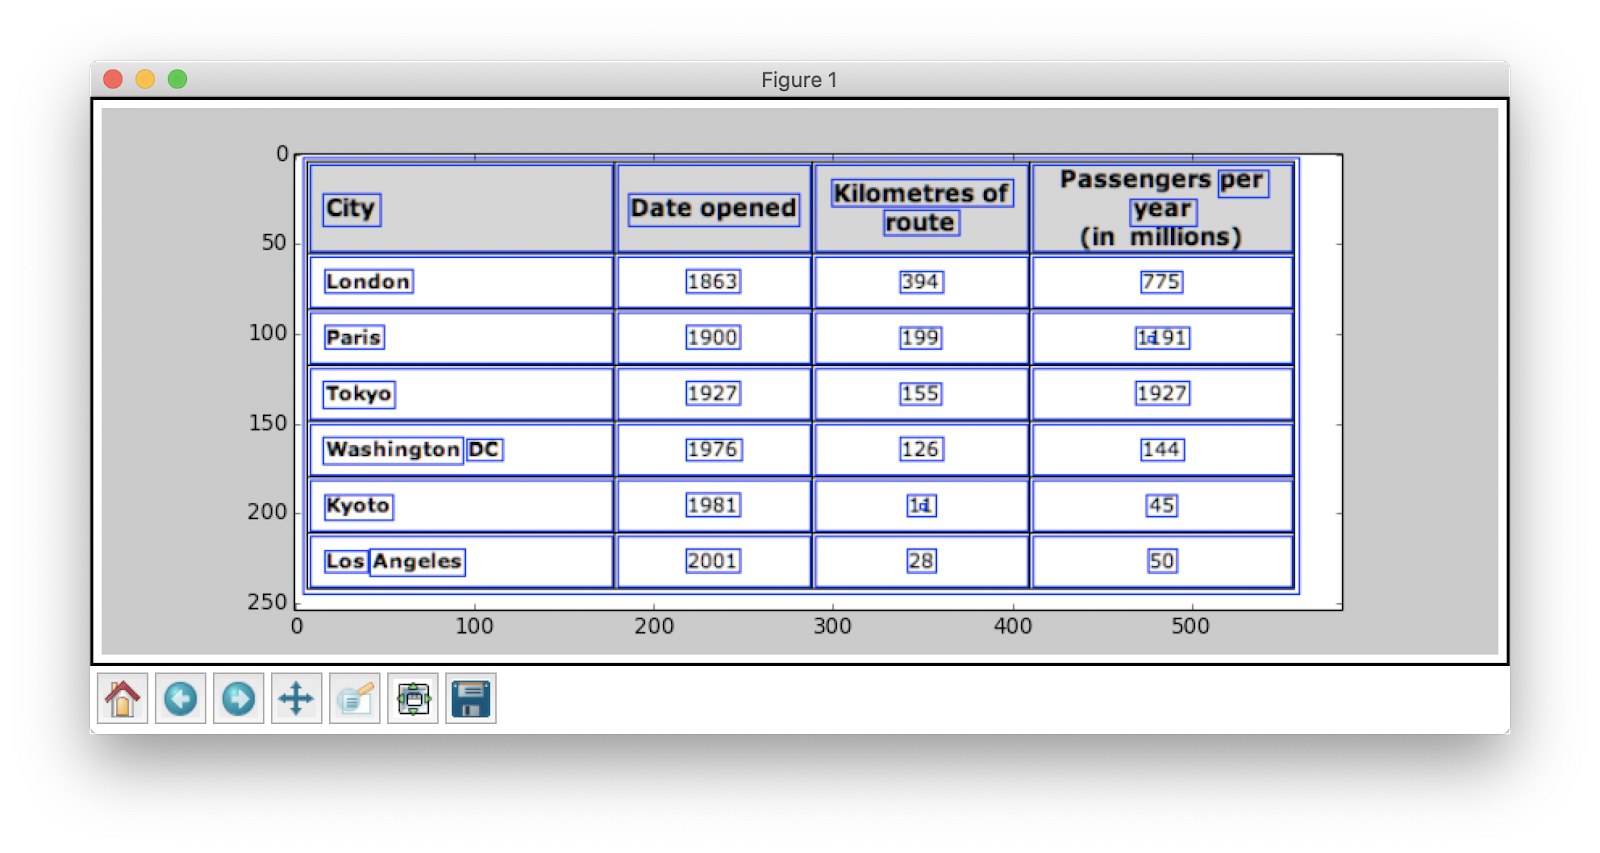
\includegraphics{assets/ocr_good.png}

}

\caption{A table that can be OCRd relatively easily}

\end{figure}

\begin{itemize}
\tightlist
\item
  Computer written text
\item
  Clean lines separating rows and columnss
\item
  Single heading per column
\end{itemize}

\hypertarget{what-does-off-the-shelf-ocr-tech-struggle-with}{%
\subsection{What does off-the-shelf OCR tech struggle
with?}\label{what-does-off-the-shelf-ocr-tech-struggle-with}}

\begin{figure}

{\centering 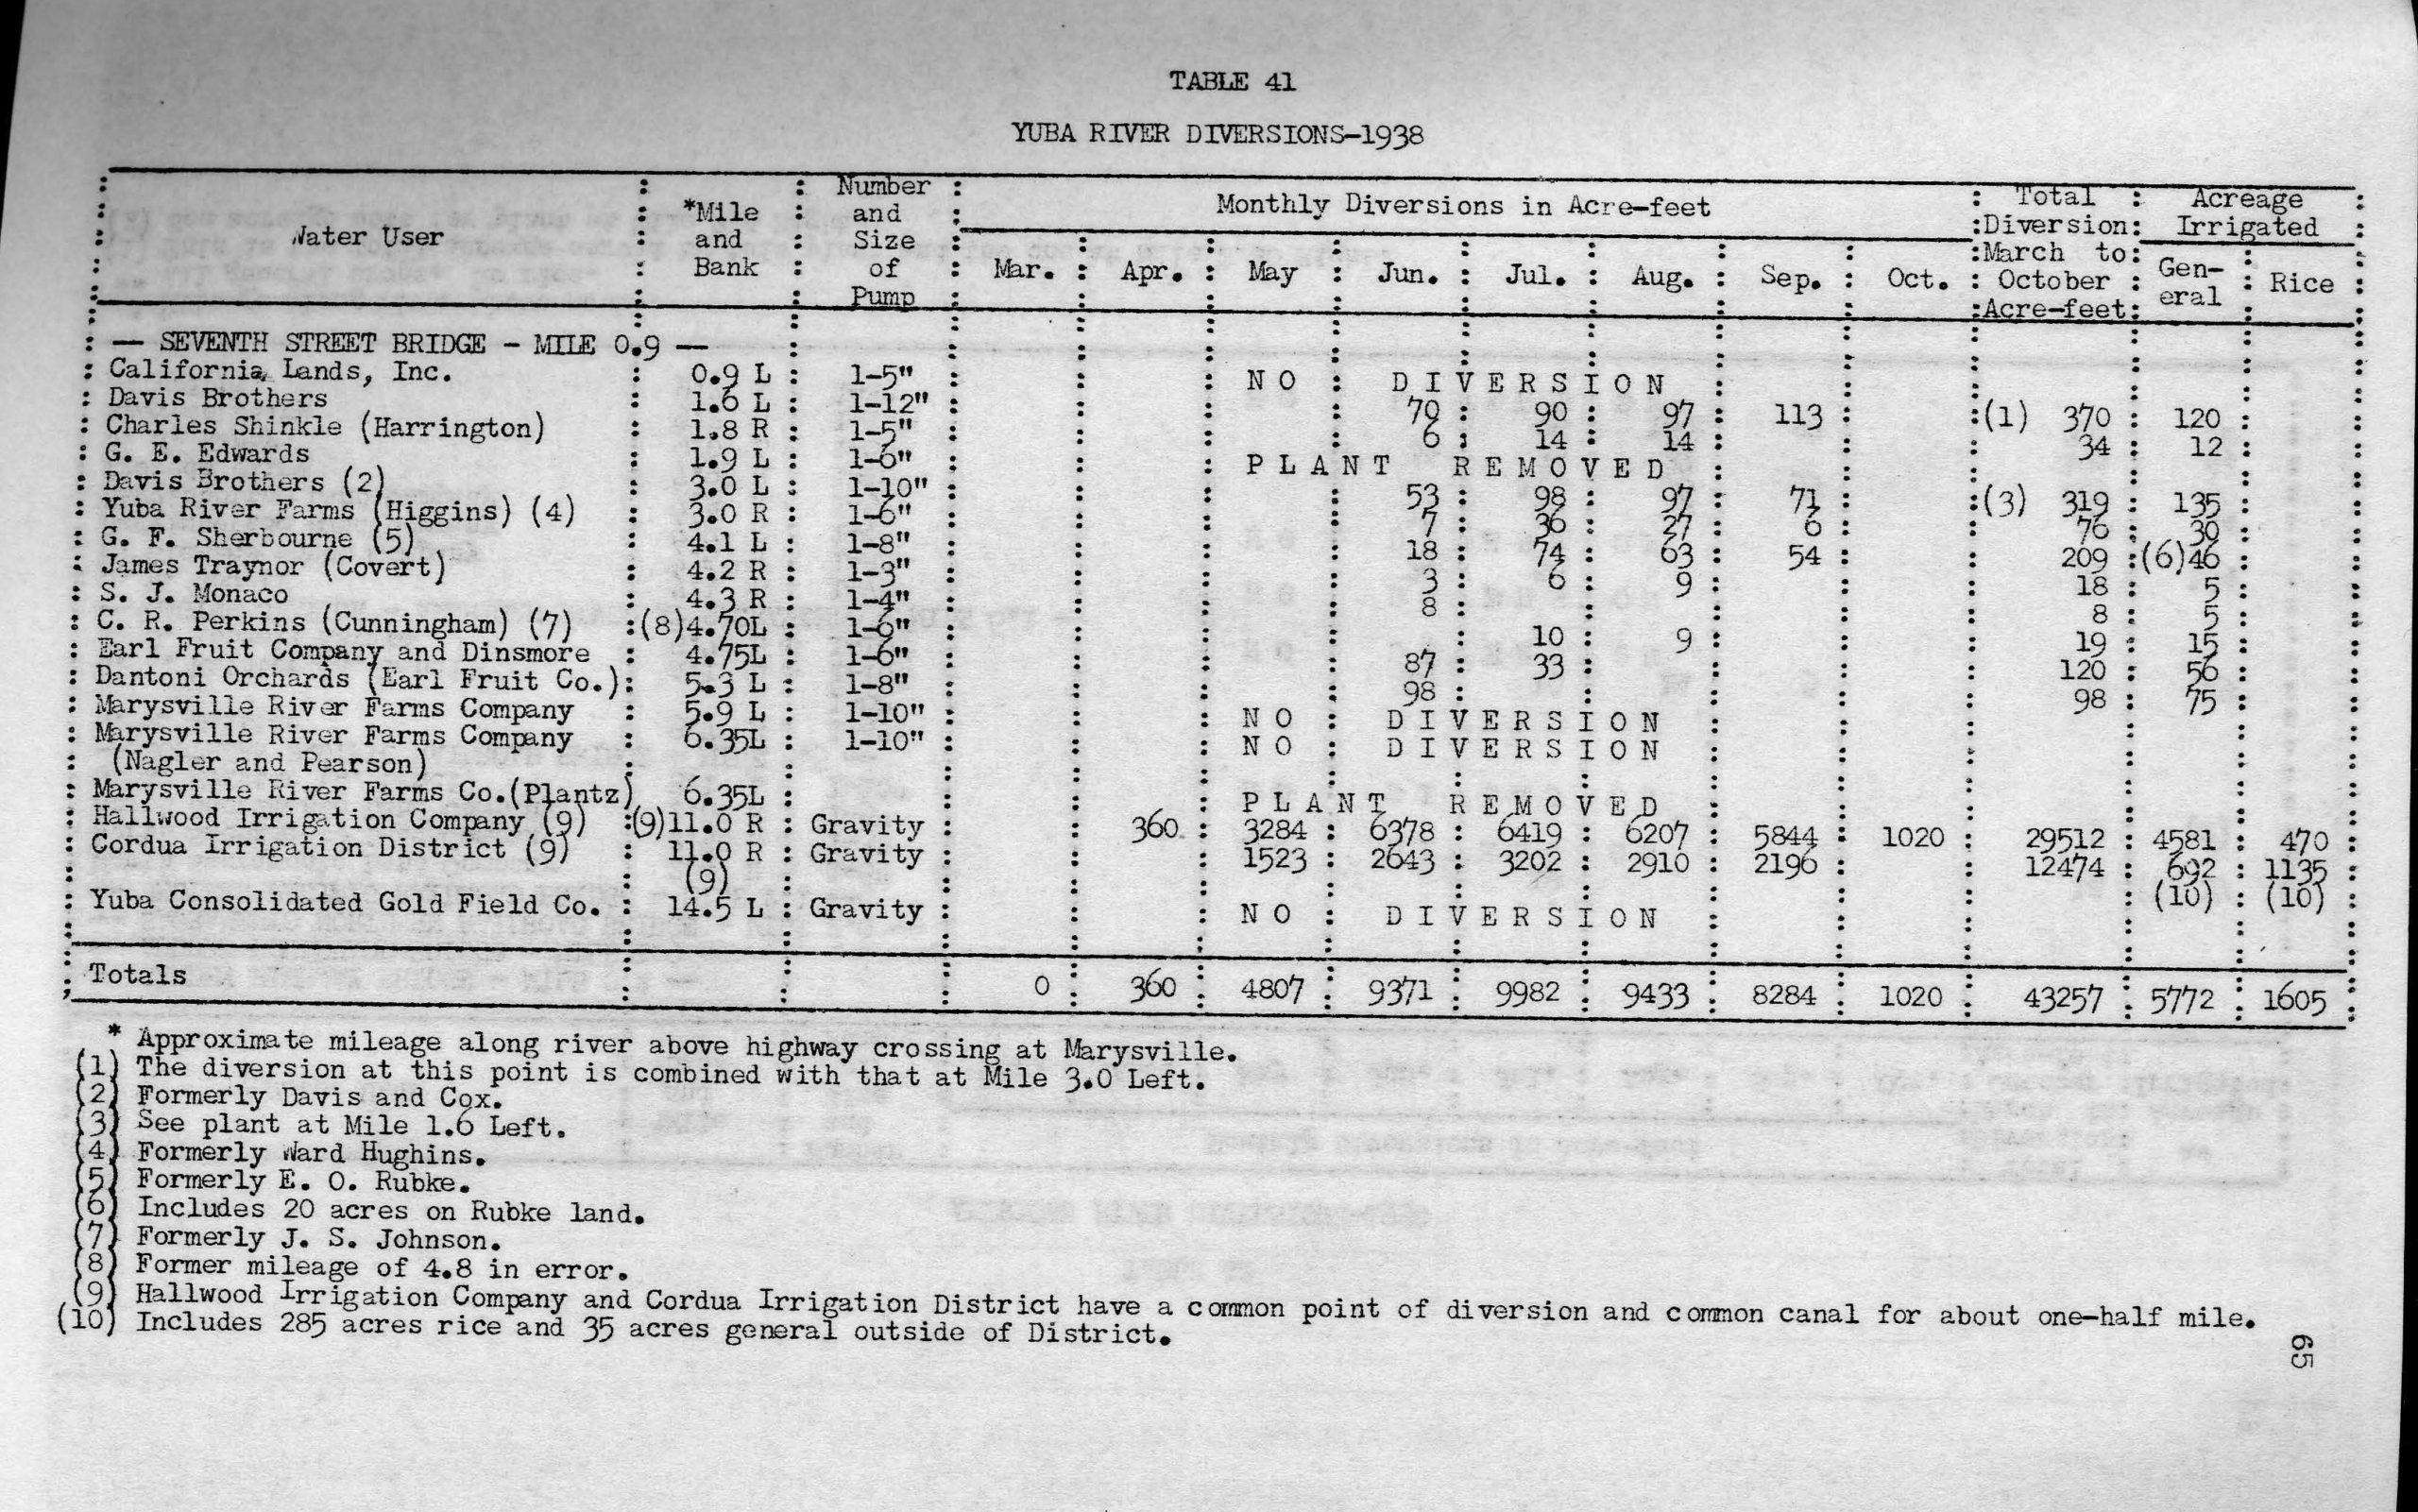
\includegraphics{assets/ocr_hard.jpg}

}

\caption{A table that is difficult to OCR}

\end{figure}

\begin{itemize}
\tightlist
\item
  Poor quality scans
\item
  Lacks clean lines separating rows
\item
  Multiple headings per column
\end{itemize}

\hypertarget{conventional-solutions-to-theses-problems}{%
\subsection{Conventional solutions to theses
problems}\label{conventional-solutions-to-theses-problems}}

\begin{figure}

{\centering 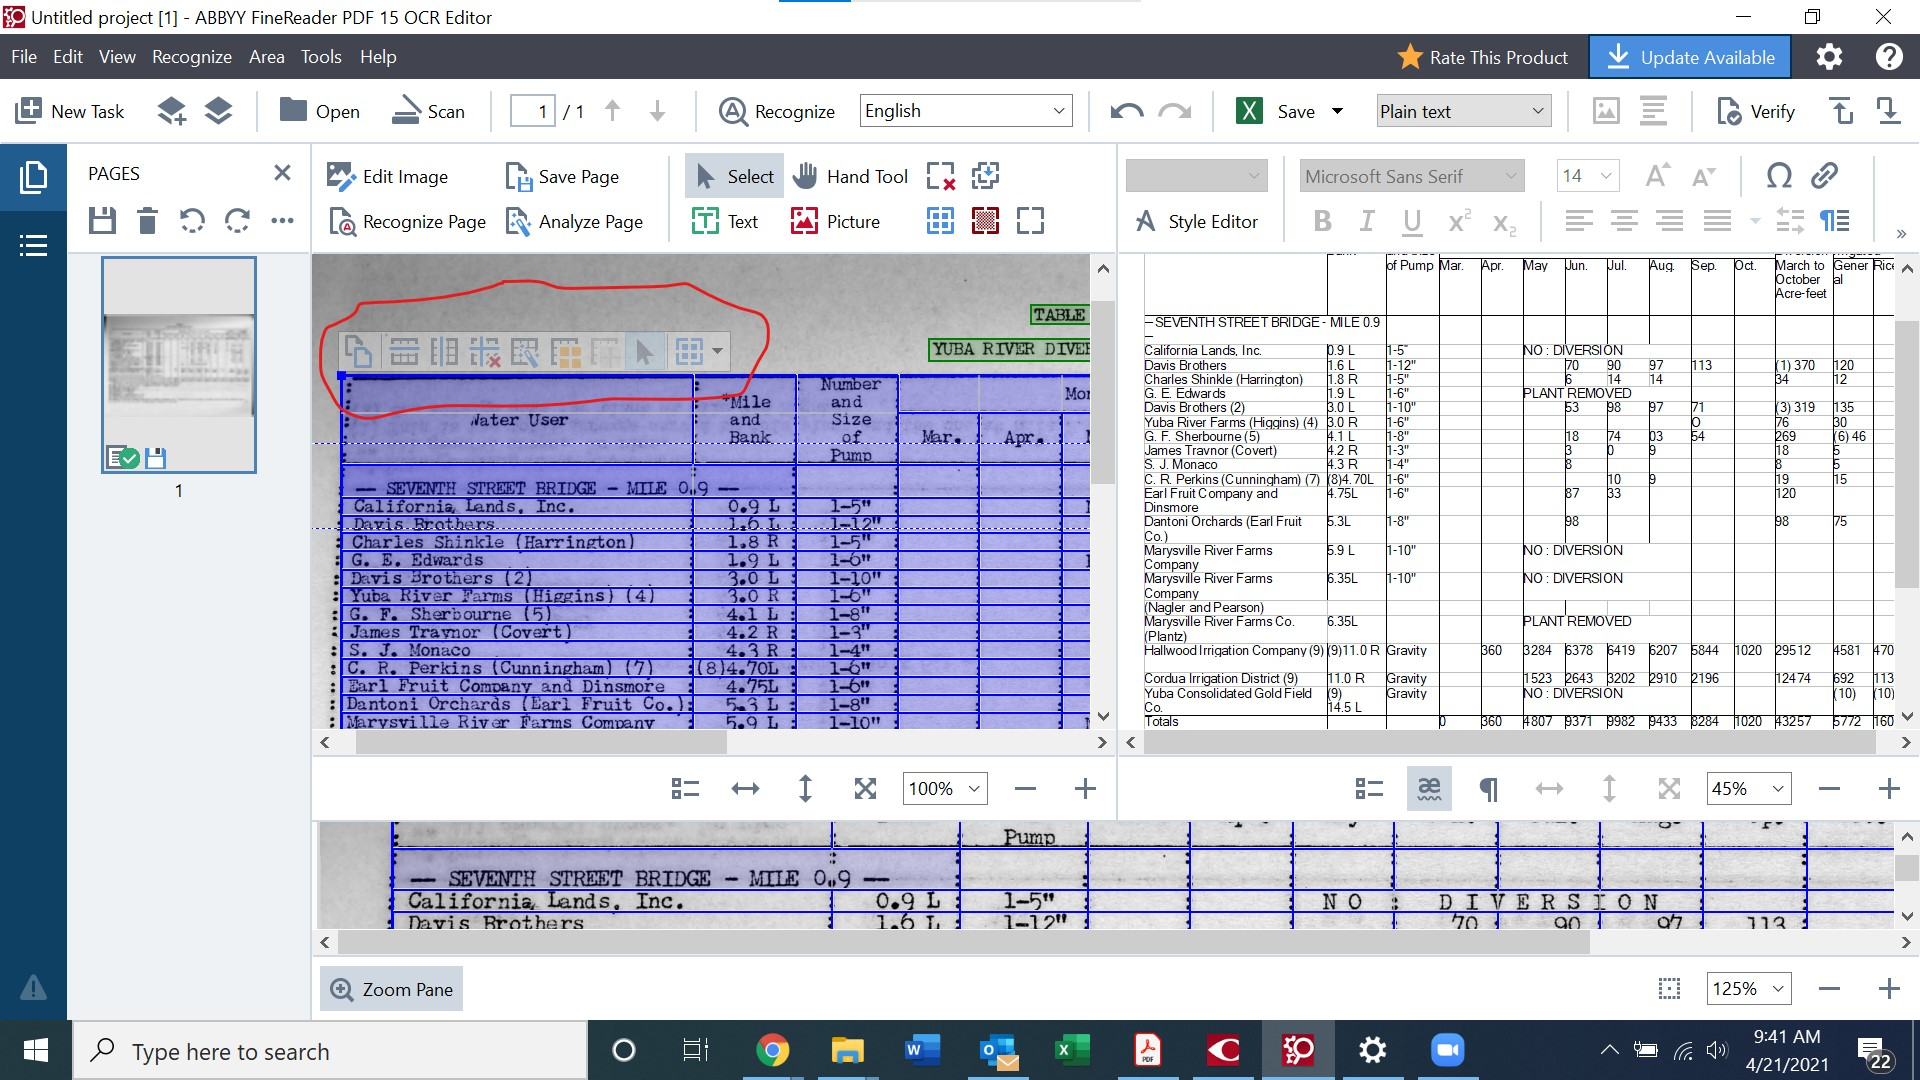
\includegraphics{assets/orc_hard_solution.jpg}

}

\caption{\href{https://bendingwater-blog.library.claremont.edu/2021/04/21/a-look-inside-the-data-ocr-process-and-challenging-tables/}{ABBYY
FineReader}}

\end{figure}

\begin{itemize}
\tightlist
\item
  Clicky, fiddly, GUI based software
\item
  Expensive
\item
  Not clear that time invested improves system
\end{itemize}

\hypertarget{custom-machine-learning-solutions}{%
\subsection{Custom machine learning
solutions}\label{custom-machine-learning-solutions}}

\begin{figure}

{\centering 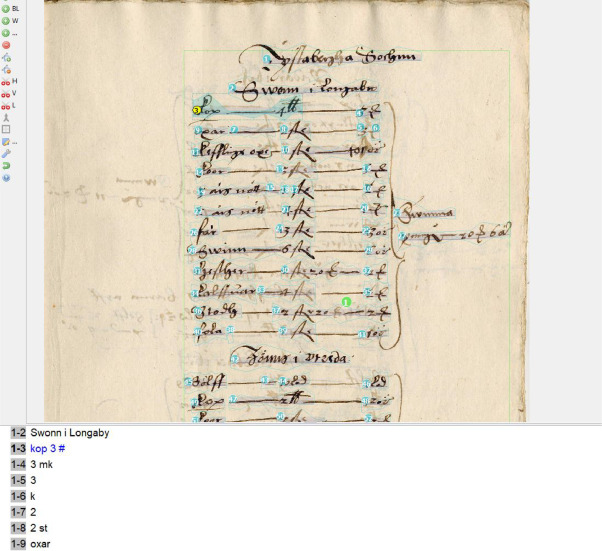
\includegraphics{assets/reading_ransom.jpg}

}

\caption{\href{}{Reading the ransom: Methodological advancements in
extracting the Swedish Wealth Tax of 1571}}

\end{figure}

\begin{itemize}
\tightlist
\item
  Use machine learning to train a model to recognize specific tables
\item
  Fantastic for old documents which would be impossible to OCR otherwise
\item
  May not generalize well to other documents
\end{itemize}

\hypertarget{custom-machine-learning-solutions-1}{%
\subsection{Custom machine learning
solutions}\label{custom-machine-learning-solutions-1}}

\begin{figure}

{\centering 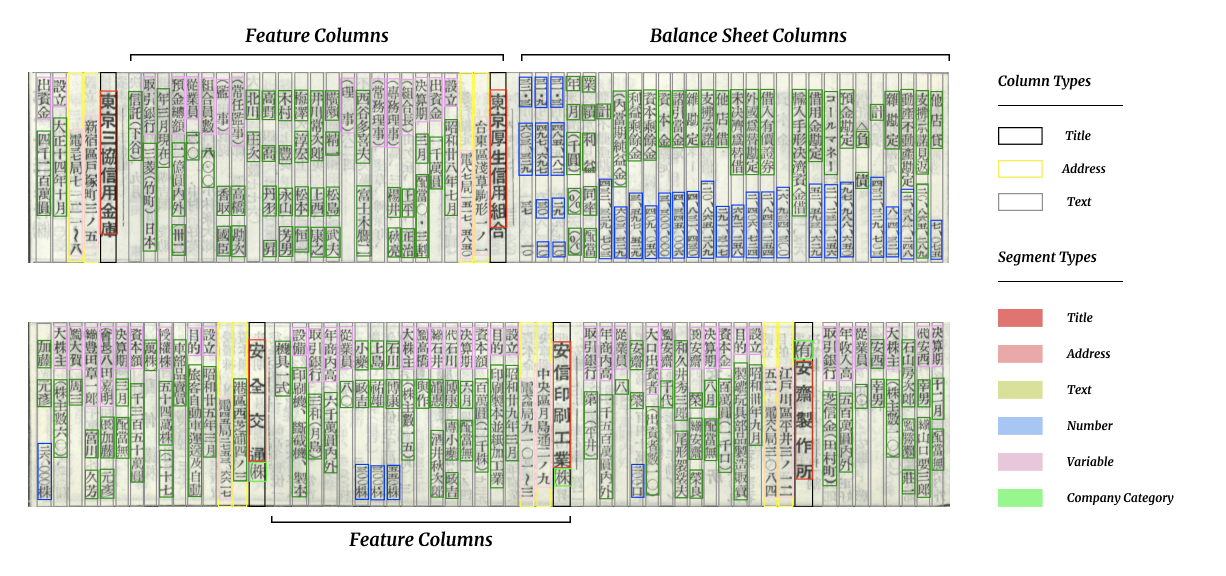
\includegraphics{assets/layout_parser.png}

}

\caption{\href{https://dell-research-harvard.github.io/resources/layout-parser}{Layout
Parser: open-source deep-learning powered library for automatically
processing document image data at scale}}

\end{figure}

\begin{itemize}
\tightlist
\item
  Use machine learning to train a model to recognize specific tables
\item
  Good for when you have a specific type of document you want to extract
  data from that doesn't change much over time
\item
  `Open source' - many open GitHub issues
\item
  You really need to know about deep learning and computer vision to use
  this well.
\end{itemize}

\hypertarget{sec-researchquestion}{%
\section{Research question}\label{sec-researchquestion}}

How can we use a multi-modal machine learning model to extract tabular
data from historical documents of varying vintages?

\hypertarget{example-use-case}{%
\subsection{Example use case:}\label{example-use-case}}

Company reports in Sweden.

I showcase the method using the annual reports of \textbf{Electrolux}, a
Swedish company founded in 1919, now the world's second largest
appliance maker by units sold.

\begin{figure}

{\centering 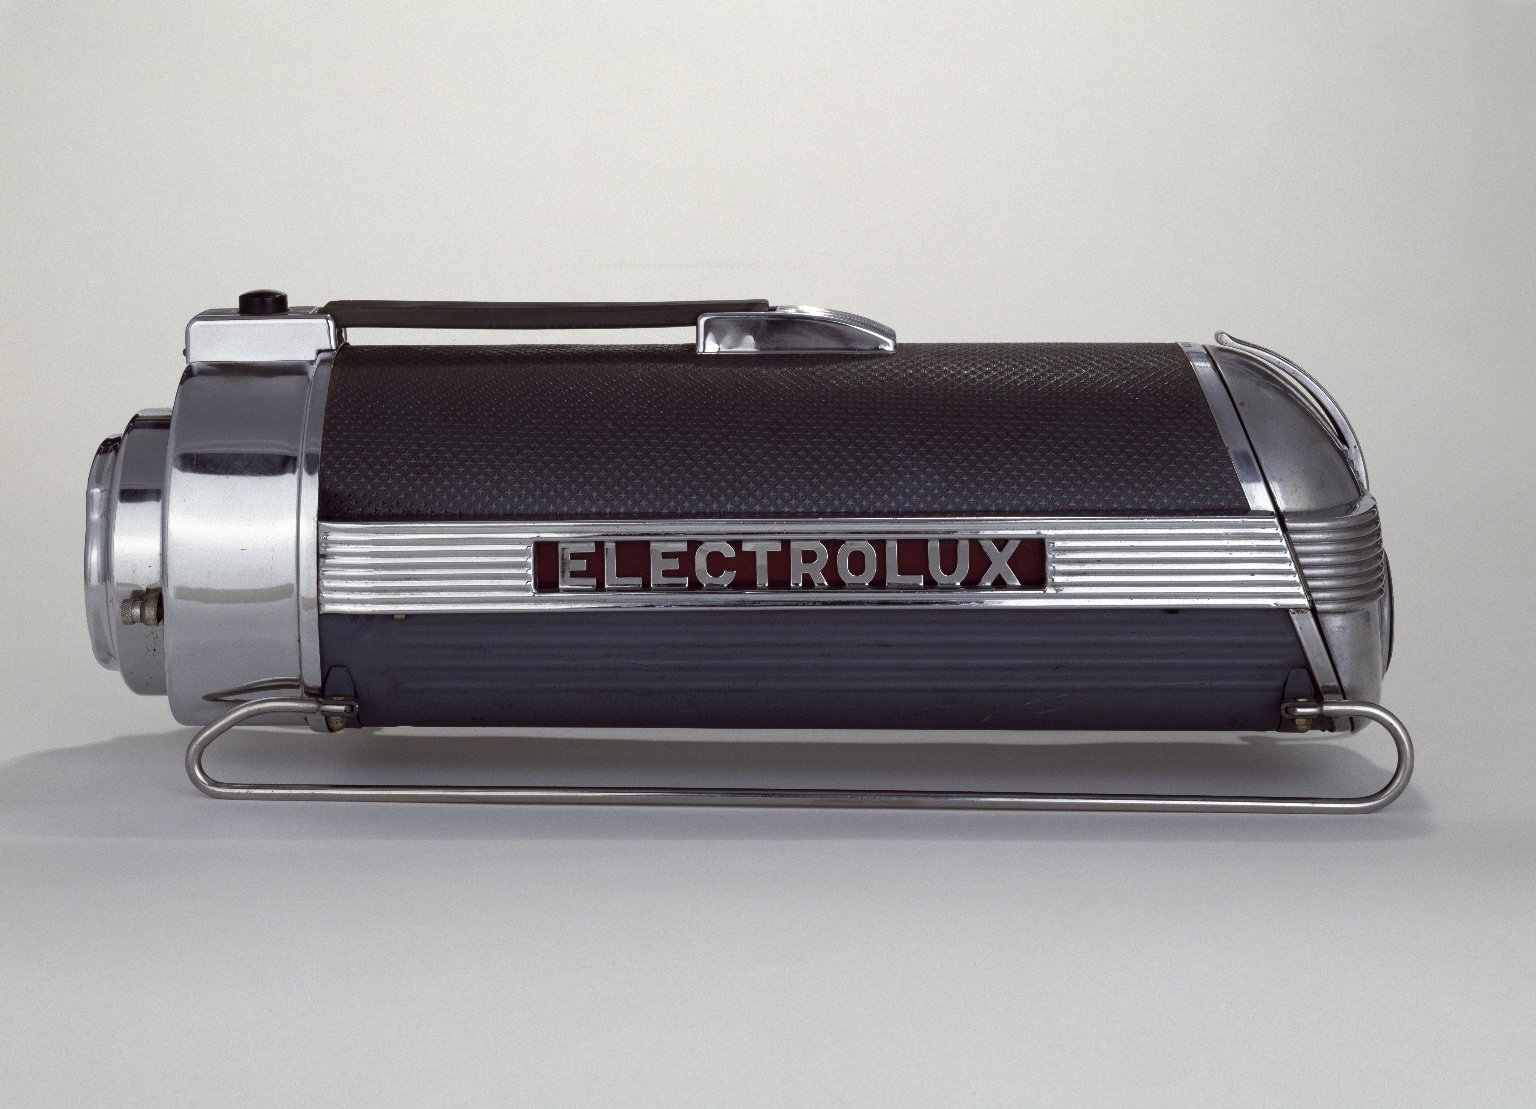
\includegraphics{assets/vacuum.jpg}

}

\caption{1937 Vacuum Cleaner}

\end{figure}

\hypertarget{source-of-data}{%
\subsection{Source of data}\label{source-of-data}}

\begin{figure}

{\centering 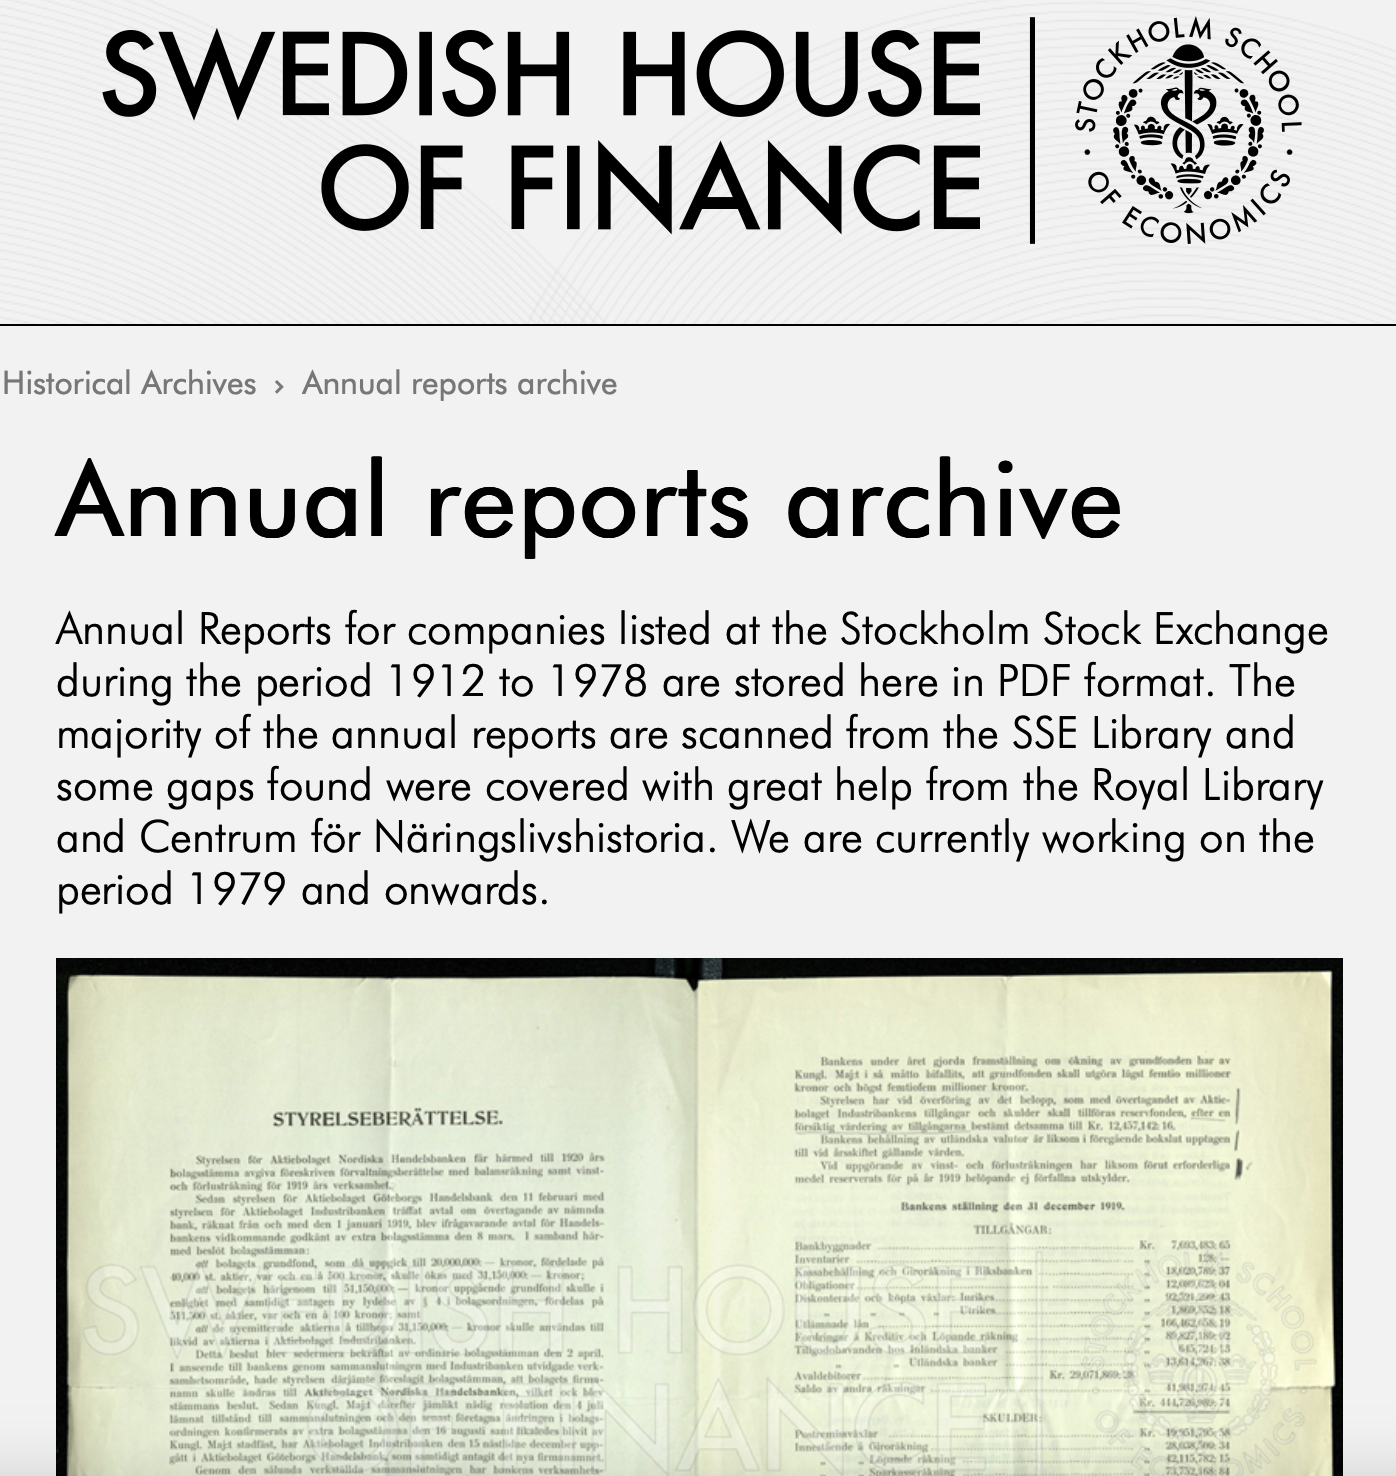
\includegraphics{assets/source_material.png}

}

\caption{\href{https://www.hhs.se/en/houseoffinance/data-center/historical-archives/annual-reports-archive/}{Annual
Reports for companies listed at the Stockholm Stock Exchange during the
period 1912 to 1978}}

\end{figure}

\hypertarget{how-do-the-reports-change-over-time}{%
\subsection{How do the reports change over
time?}\label{how-do-the-reports-change-over-time}}

\begin{verbatim}
-- Attaching core tidyverse packages ------------------------ tidyverse 2.0.0 --
v dplyr     1.1.3     v readr     2.1.4
v forcats   1.0.0     v stringr   1.5.0
v ggplot2   3.4.4     v tibble    3.2.1
v lubridate 1.9.3     v tidyr     1.3.0
v purrr     1.0.2     
-- Conflicts ------------------------------------------ tidyverse_conflicts() --
x dplyr::filter() masks stats::filter()
x dplyr::lag()    masks stats::lag()
i Use the conflicted package (<http://conflicted.r-lib.org/>) to force all conflicts to become errors
New names:
Rows: 76 Columns: 2
-- Column specification --------------------------------------------------------
Delimiter: ","
dbl (2): ...1, pages

i Use `spec()` to retrieve the full column specification for this data.
i Specify the column types or set `show_col_types = FALSE` to quiet this message.
\end{verbatim}

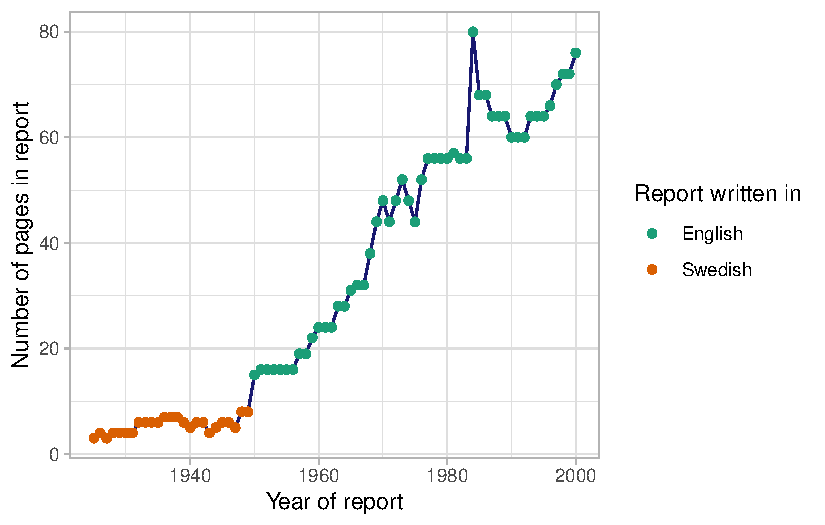
\includegraphics{index_files/figure-pdf/unnamed-chunk-1-1.pdf}

\hypertarget{reports-over-time}{%
\subsection{Reports over time}\label{reports-over-time}}

\begin{figure}

\begin{minipage}[t]{0.33\linewidth}

{\centering 

\raisebox{-\height}{

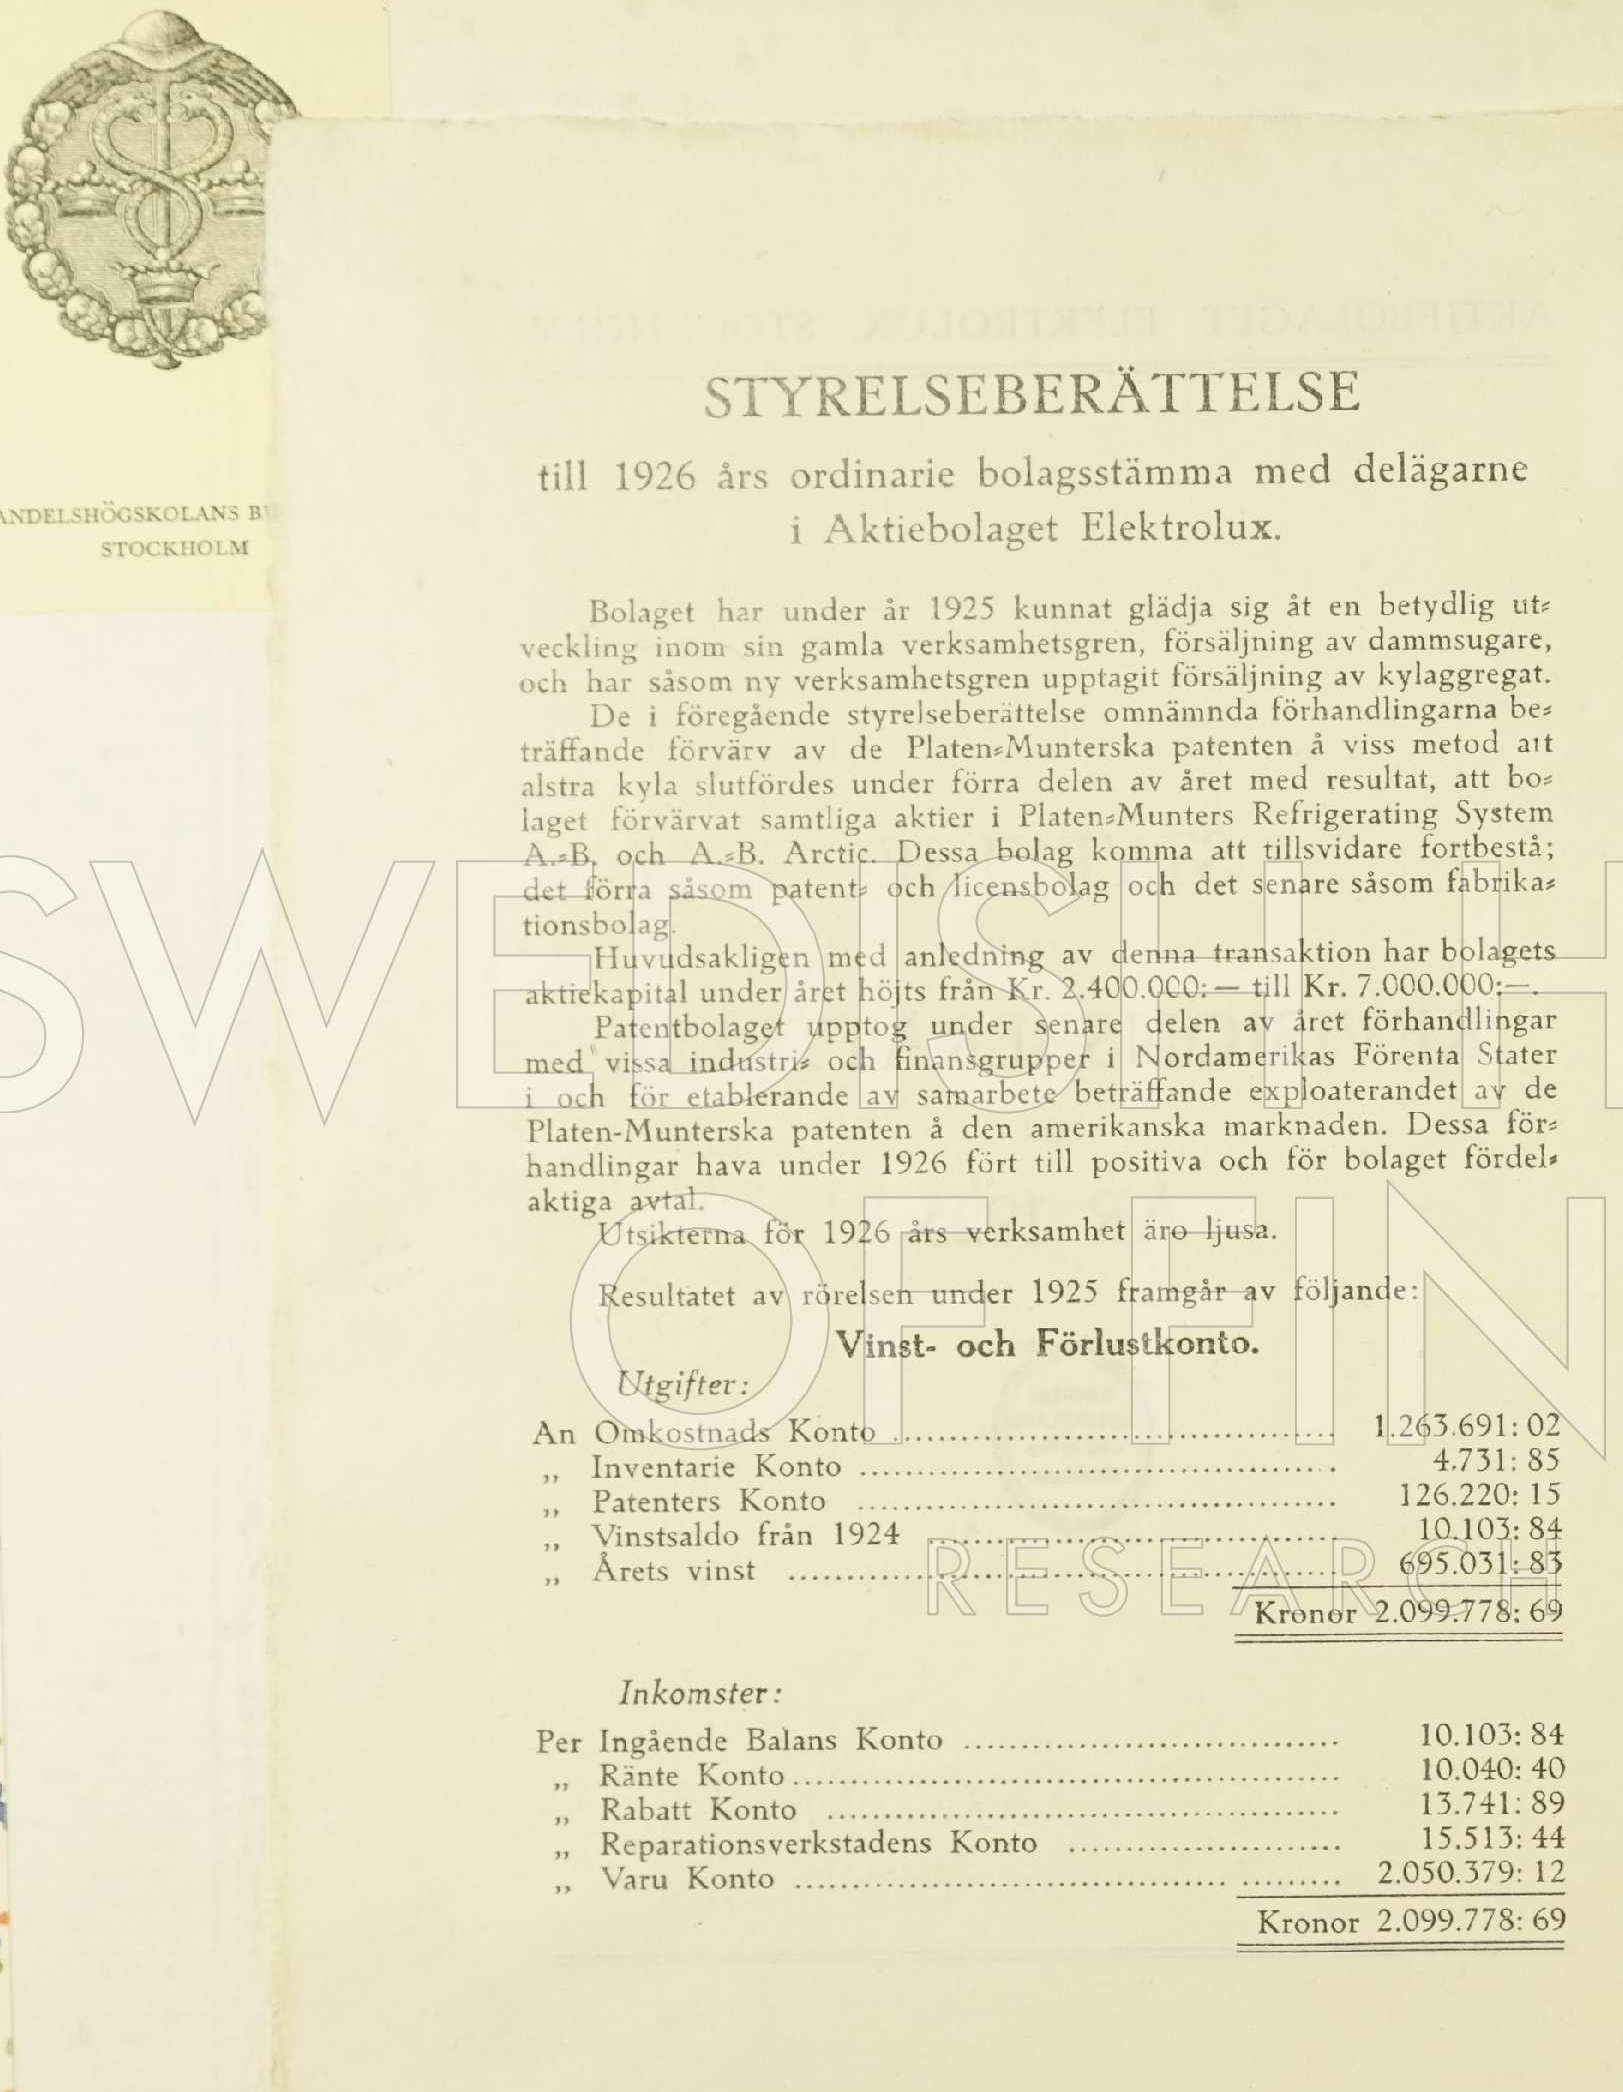
\includegraphics{assets/1925_crop.png}

}

\caption{1925}

}

\end{minipage}%
%
\begin{minipage}[t]{0.33\linewidth}

{\centering 

\raisebox{-\height}{

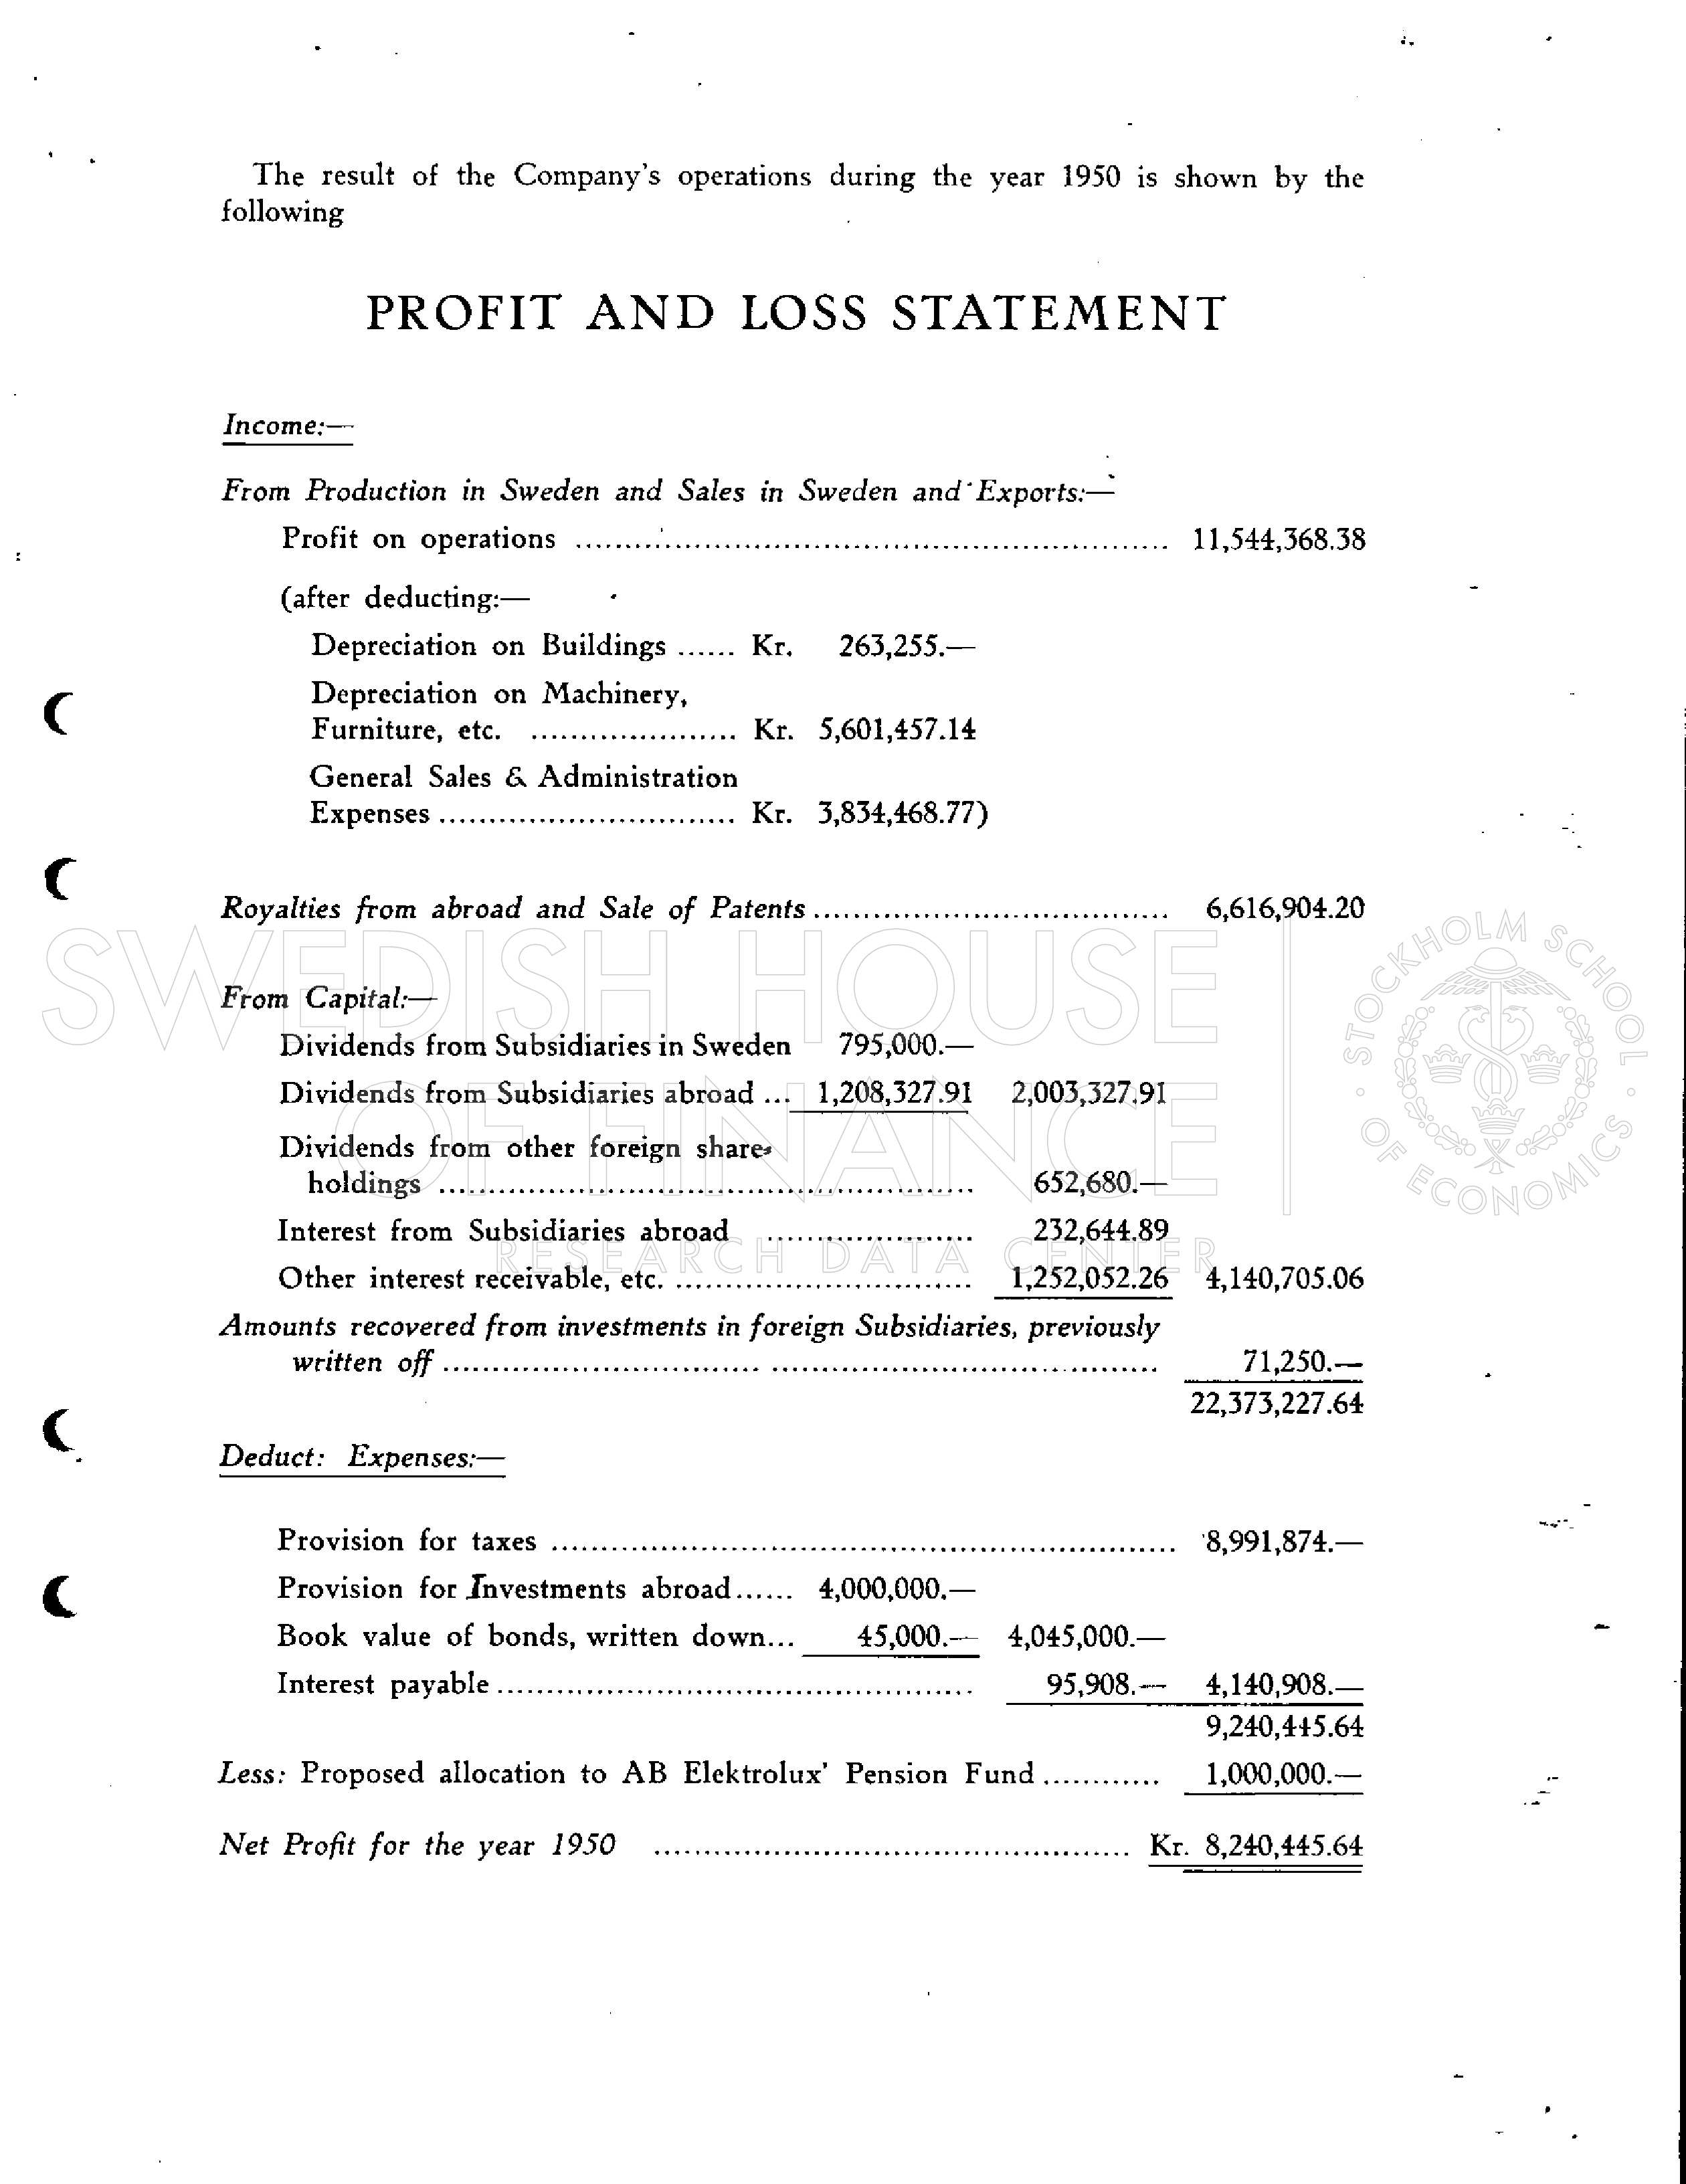
\includegraphics{data/companies/Electrolux/1950/single_pages/Electrolux_1950_page_5.jpeg}

}

\caption{1950}

}

\end{minipage}%
%
\begin{minipage}[t]{0.33\linewidth}

{\centering 

\raisebox{-\height}{

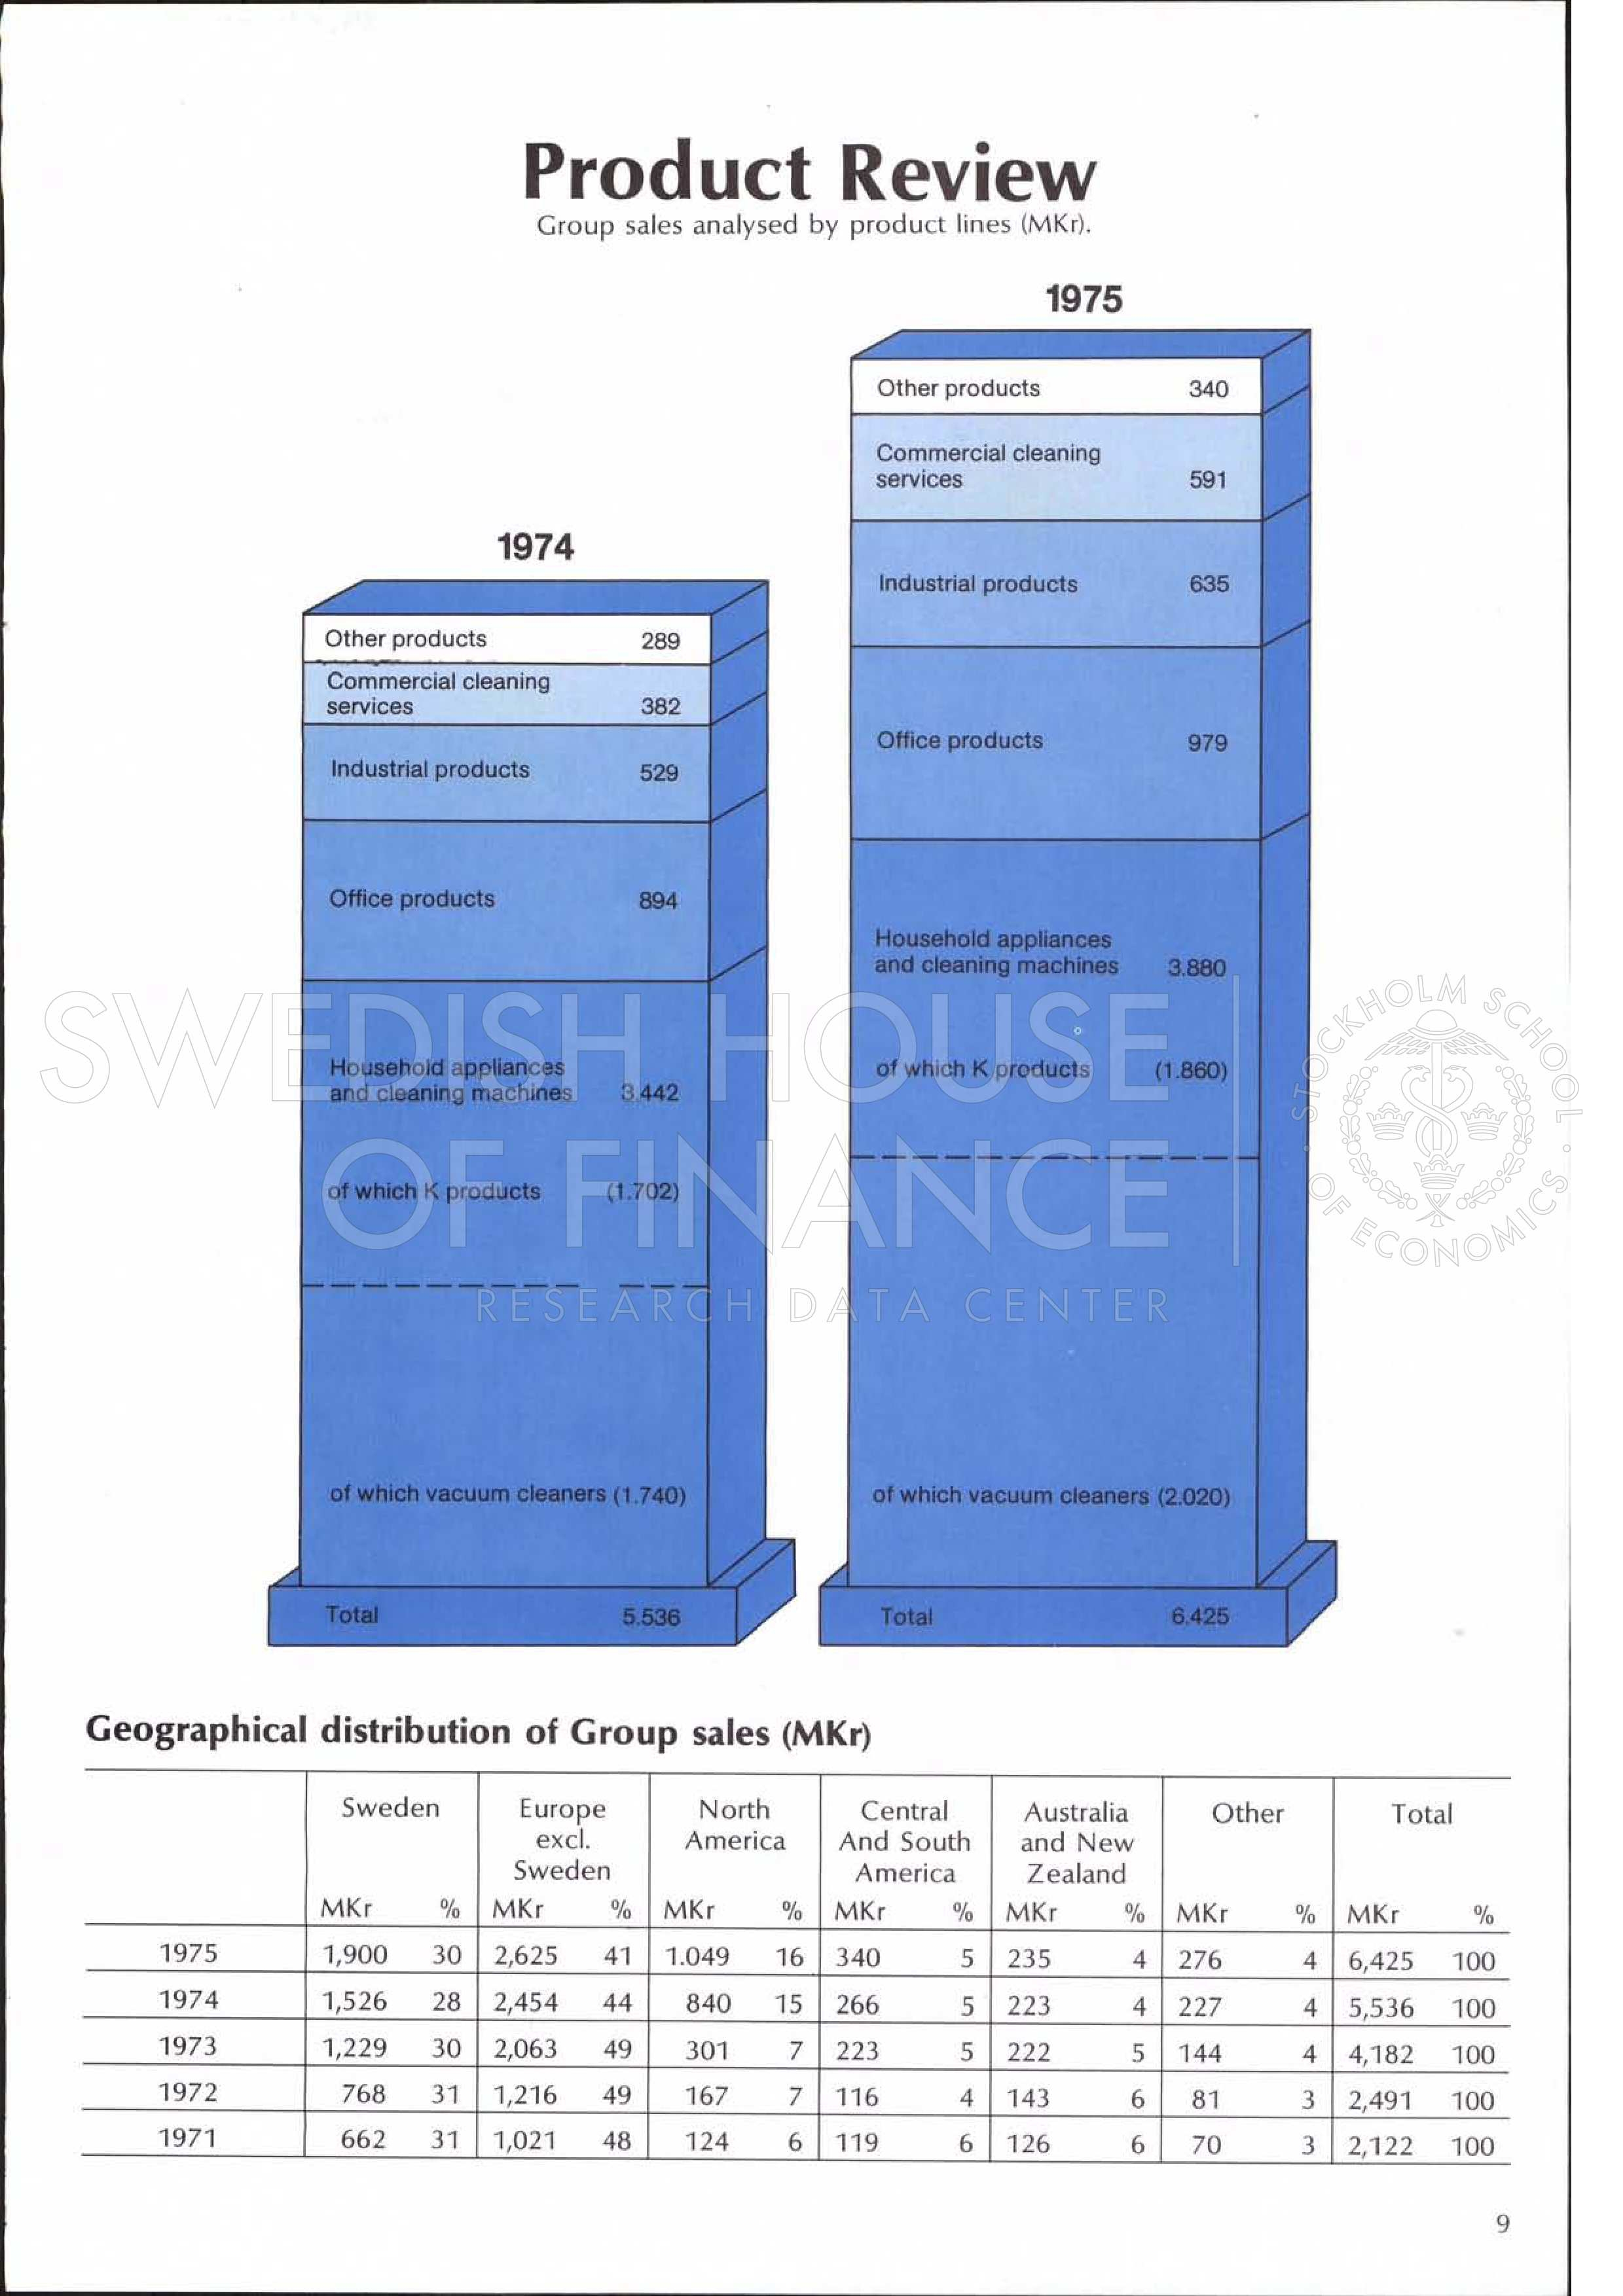
\includegraphics{data/companies/Electrolux/1975/single_pages/Electrolux_1975_page_11.jpeg}

}

\caption{1975}

}

\end{minipage}%

\end{figure}

\hypertarget{reports-over-time-graphic-design}{%
\subsection{Reports over time: GRAPHIC
DESIGN!}\label{reports-over-time-graphic-design}}

\begin{figure}

\begin{minipage}[t]{0.33\linewidth}

{\centering 

\raisebox{-\height}{

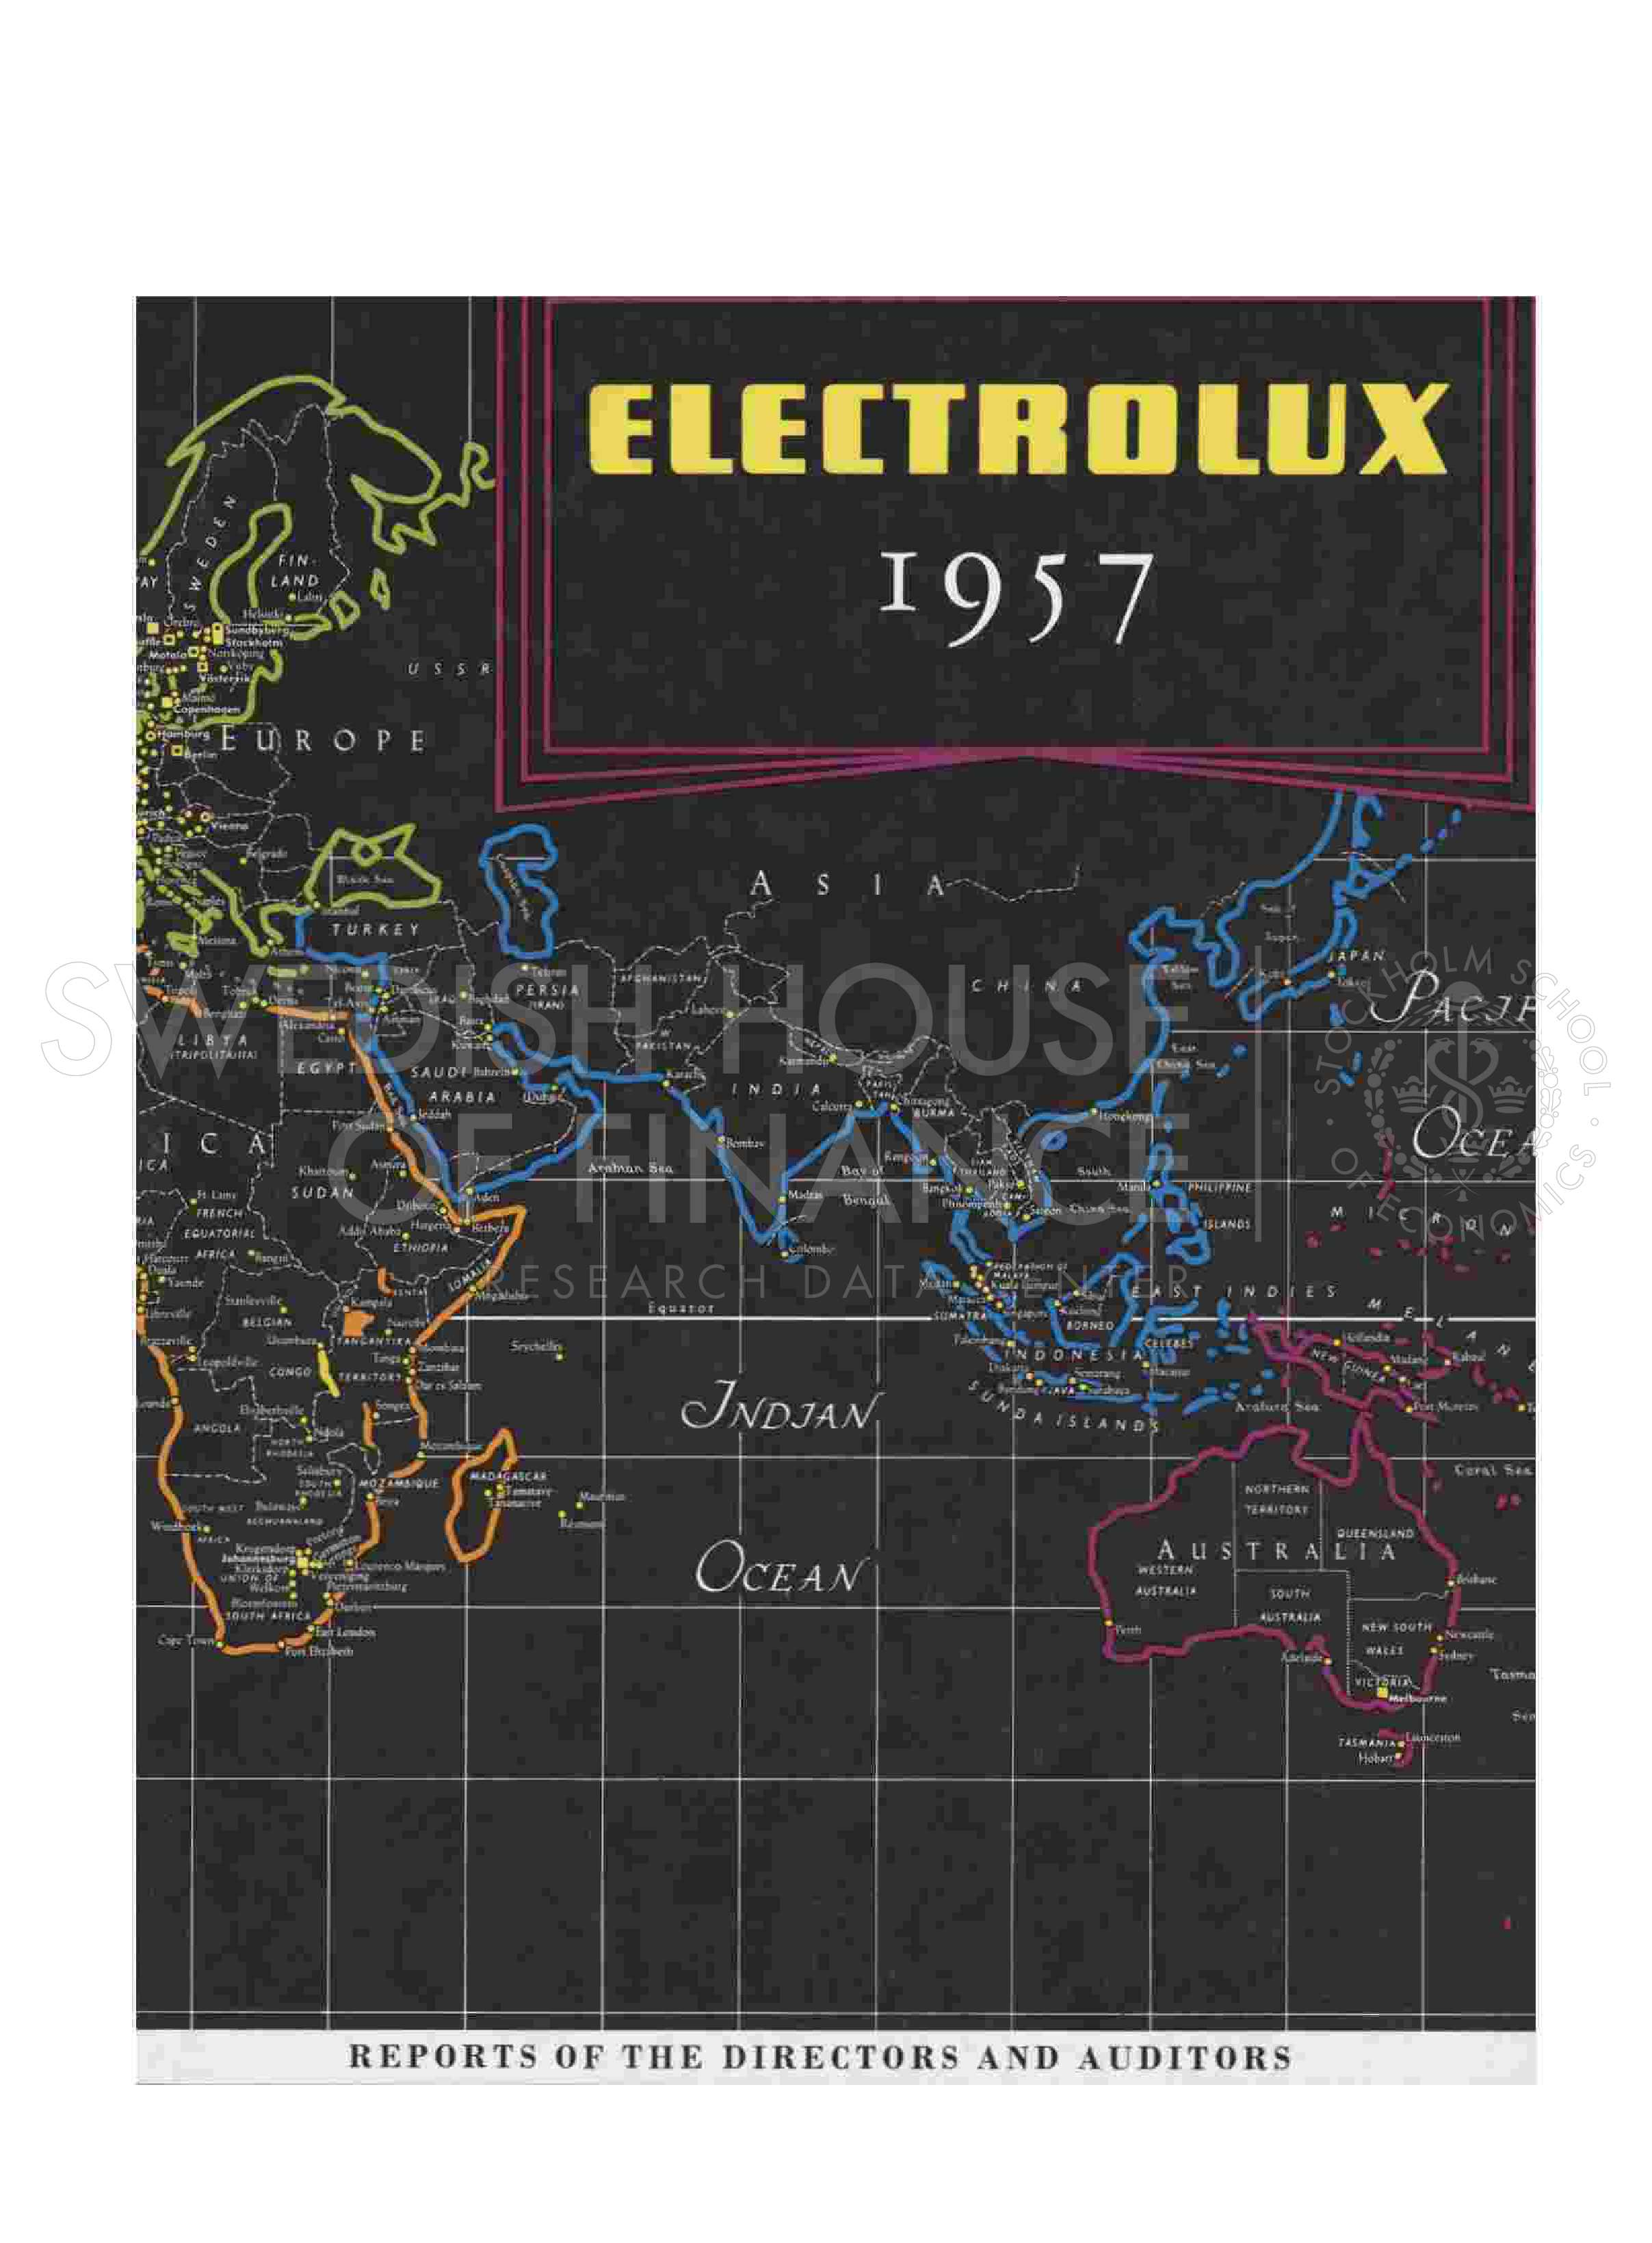
\includegraphics{data/companies/Electrolux/1957/single_pages/Electrolux_1957_page_1.jpeg}

}

\caption{1957}

}

\end{minipage}%
%
\begin{minipage}[t]{0.33\linewidth}

{\centering 

\raisebox{-\height}{


\includegraphics{data/companies/Electrolux/1972/single_pages/Electrolux_1972_page_1.jpeg}

}

\caption{1972}

}

\end{minipage}%
%
\begin{minipage}[t]{0.33\linewidth}

{\centering 

\raisebox{-\height}{

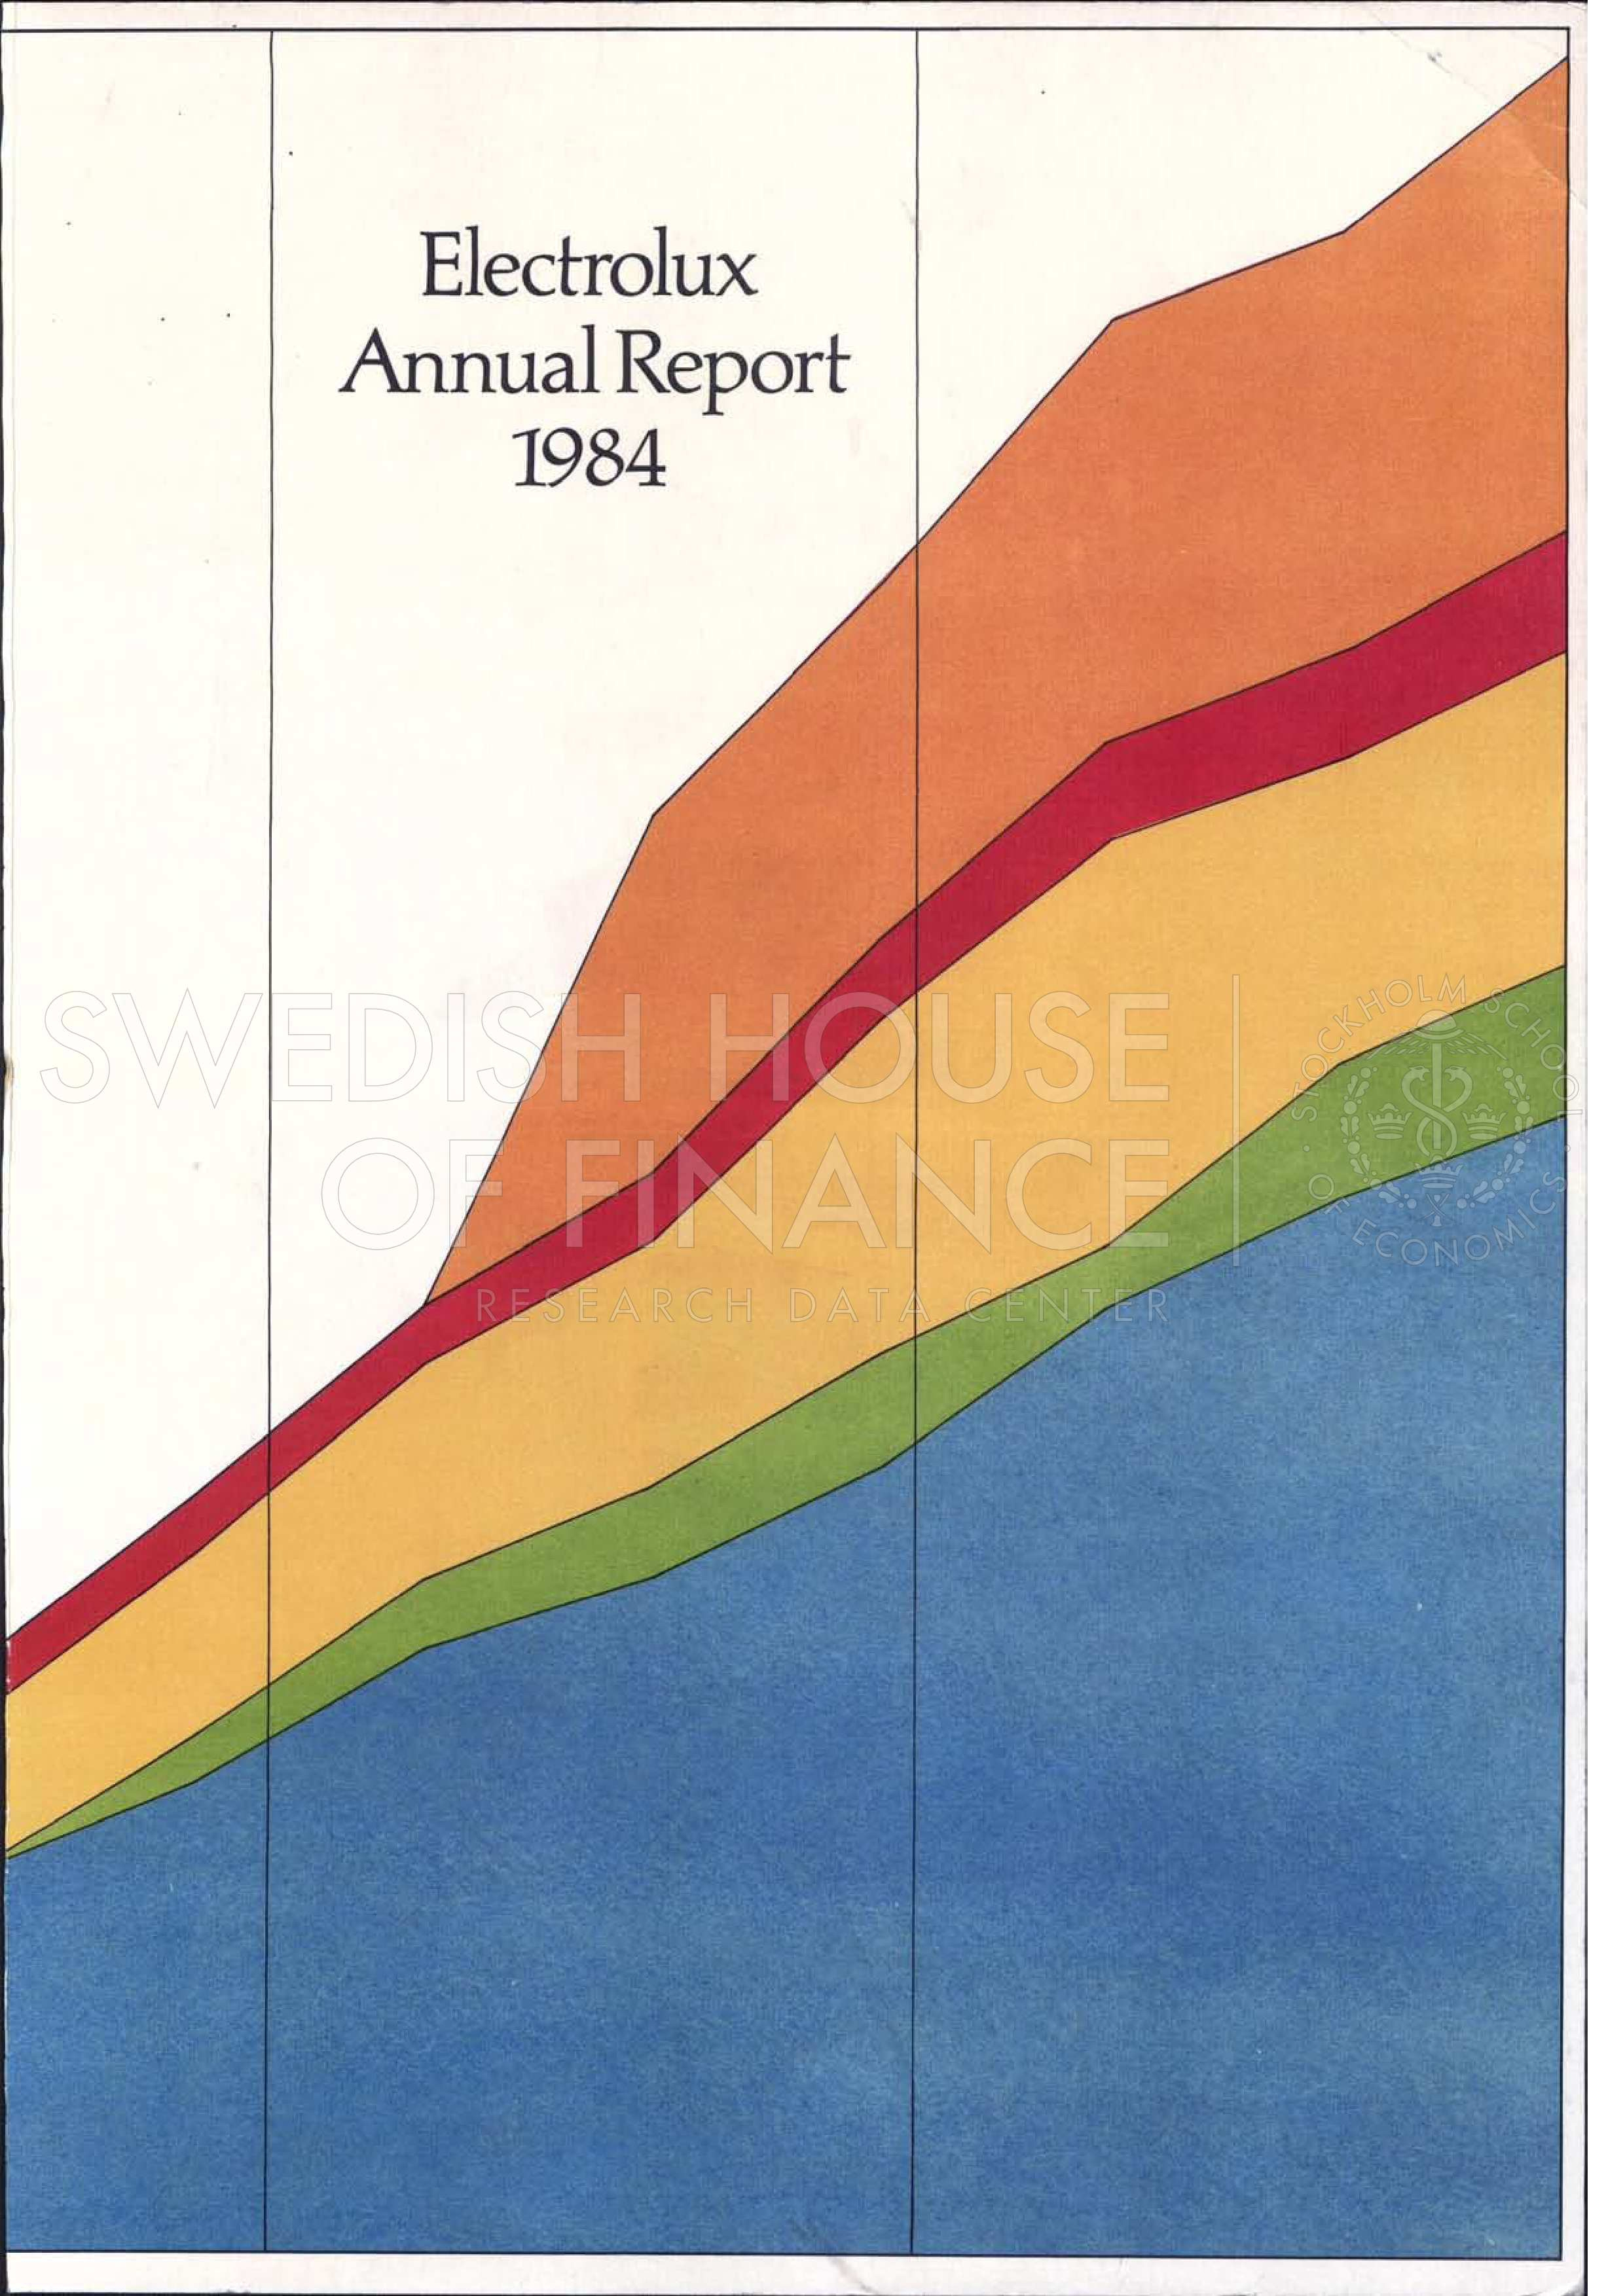
\includegraphics{data/companies/Electrolux/1984/single_pages/Electrolux_1984_page_1.jpeg}

}

\caption{1984}

}

\end{minipage}%

\end{figure}

\hypertarget{sec-approach}{%
\section{Approach}\label{sec-approach}}

Combination of vector database for document search and multi-modal
machine learning for table extraction.

\hypertarget{approach-schematic}{%
\subsection{Approach schematic}\label{approach-schematic}}

\begin{figure}

{\centering 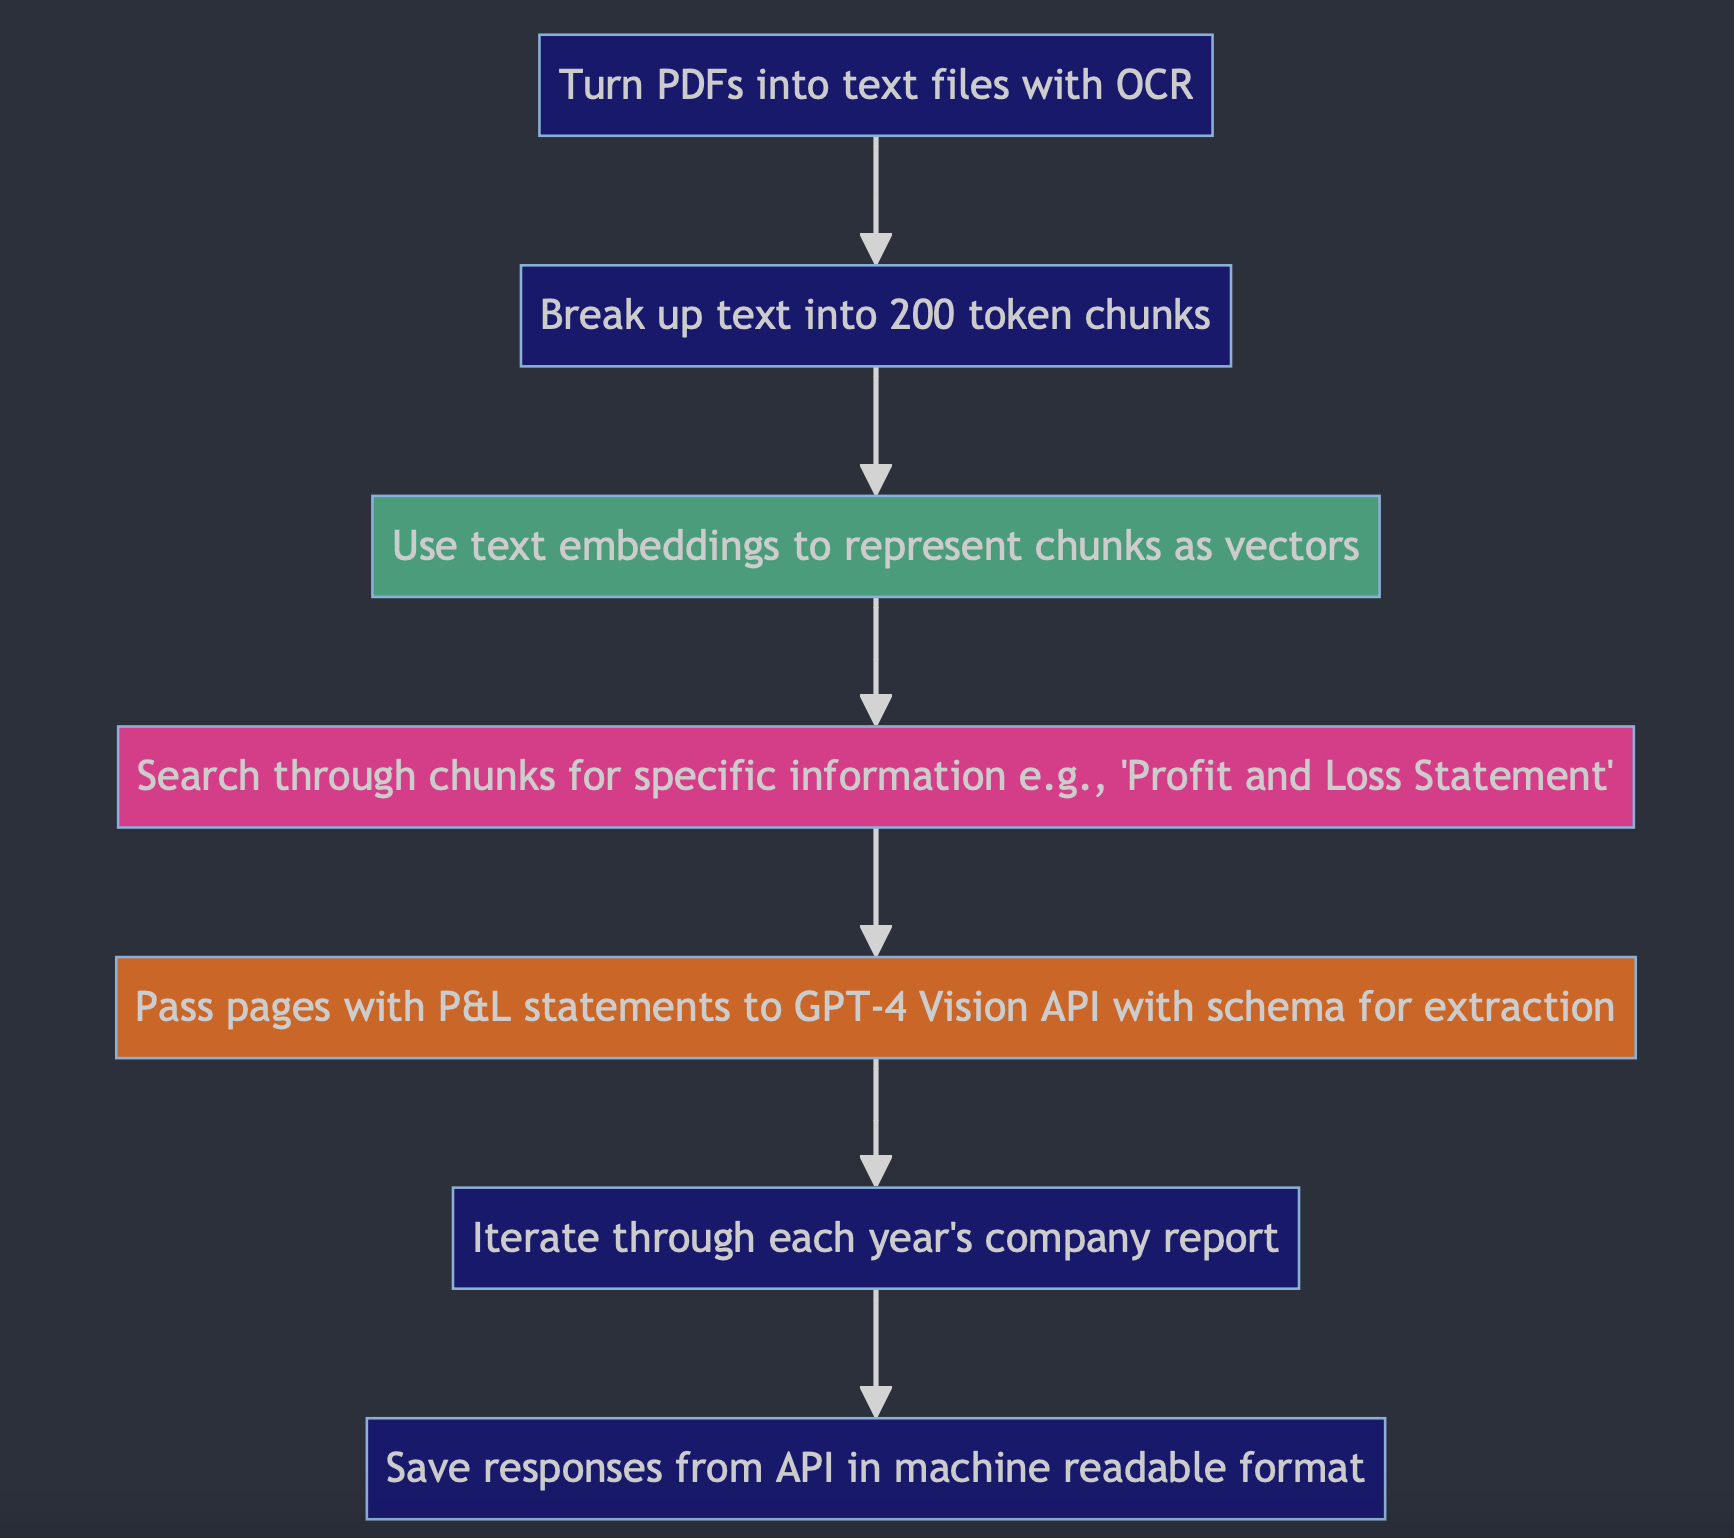
\includegraphics{assets/mermaid.png}

}

\caption{How we get information out of tabular PDFs}

\end{figure}

\hypertarget{semantic-search-explained}{%
\subsection{Semantic search explained}\label{semantic-search-explained}}

\begin{figure}

{\centering 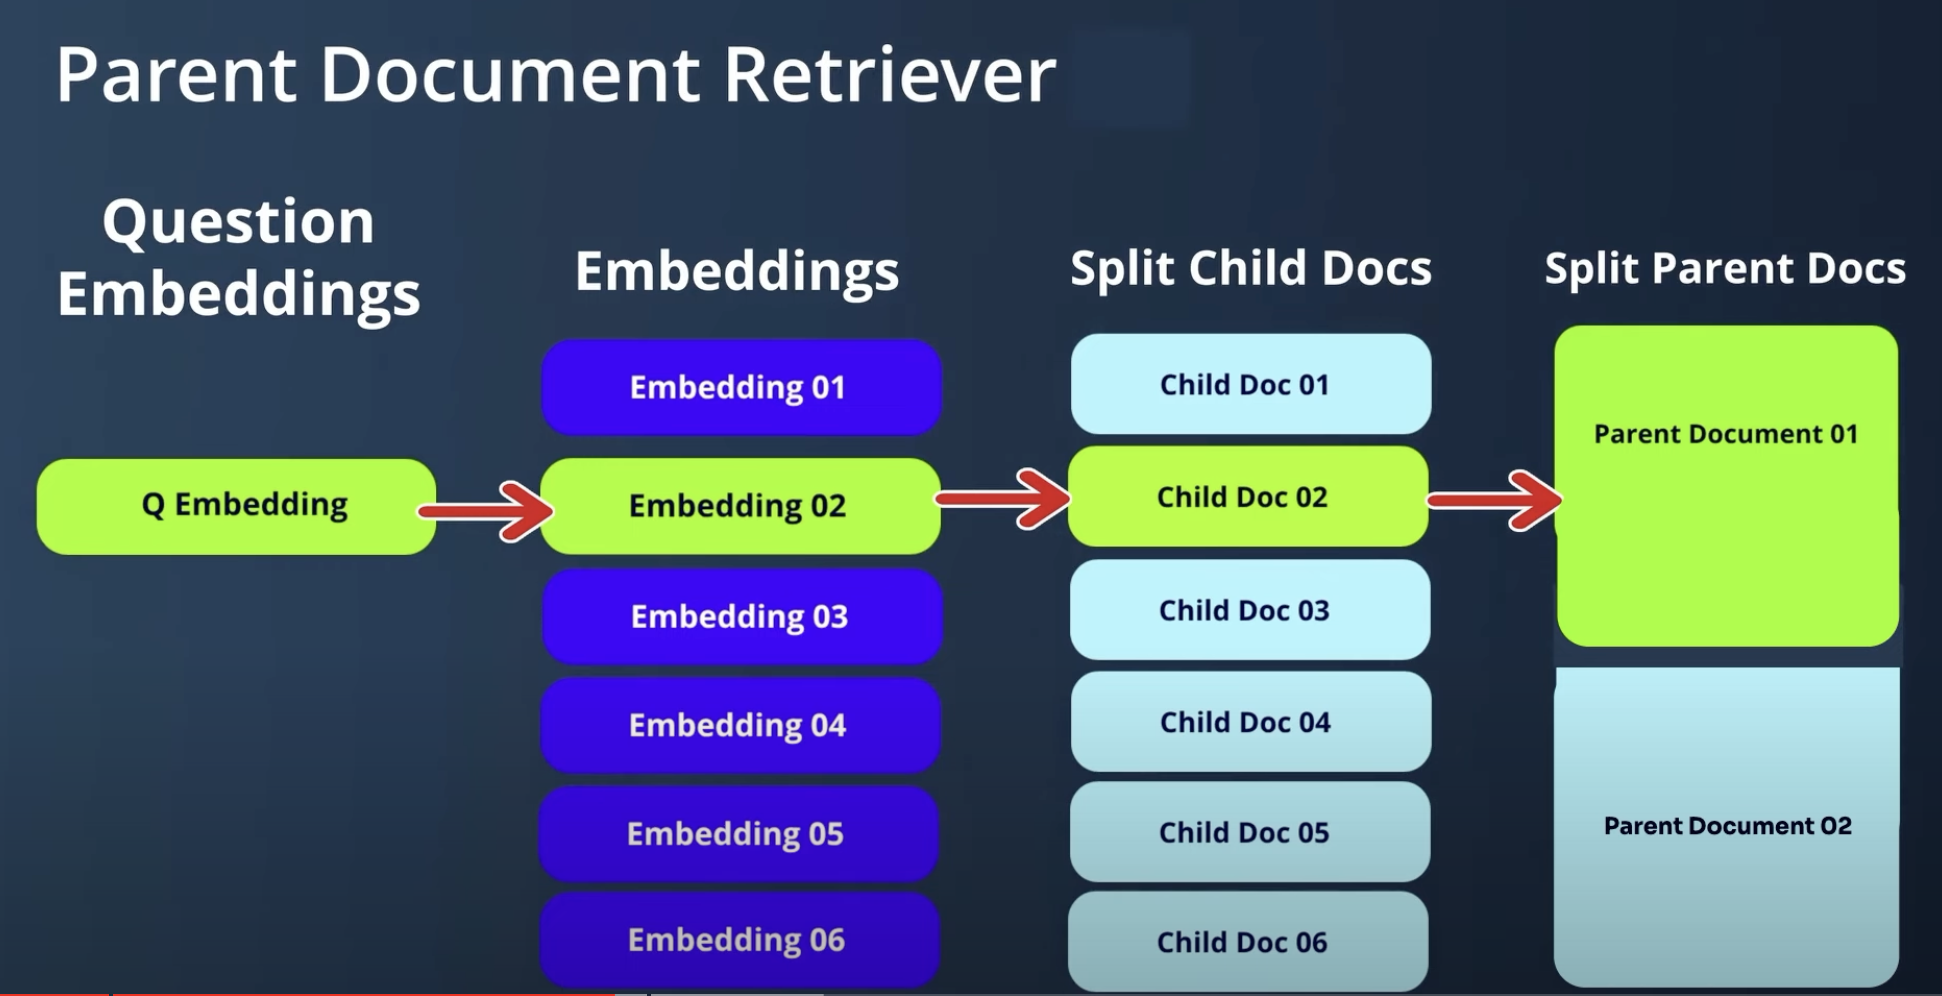
\includegraphics{assets/parent-document-retriever.png}

}

\caption{Search process}

\end{figure}

\hypertarget{use-text-embeddings-to-represent-chunks-as-vectors}{%
\subsection{Use text embeddings to represent chunks as
vectors}\label{use-text-embeddings-to-represent-chunks-as-vectors}}

``Vinst- och förlusträkning'' \textasciitilde{} {[}1, 0, 1, 0, 0,
\ldots{]} \textasciitilde{} ``Profit and loss account''

Then we find the page of the document that contains the Profit and Loss
account.

\begin{verbatim}
Warning: Removed 30 rows containing missing values (`geom_point()`).
\end{verbatim}

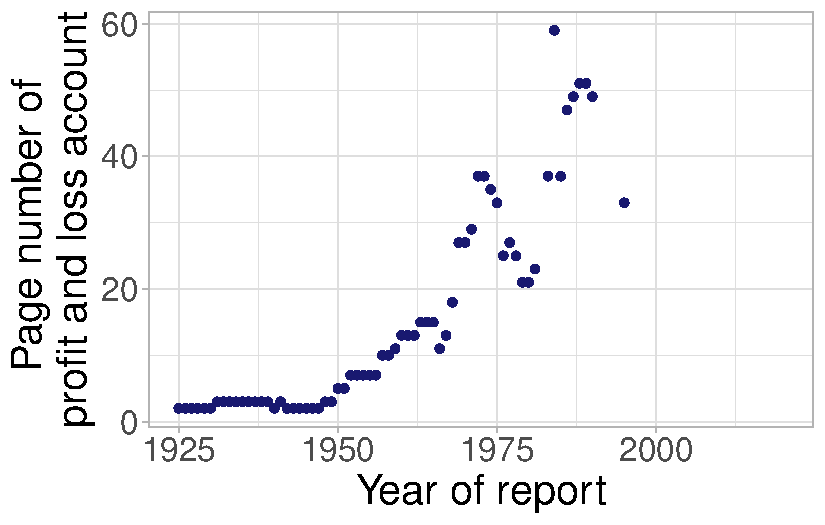
\includegraphics{index_files/figure-pdf/unnamed-chunk-2-1.pdf}

\emph{The National Library of Sweden / KBLab released three pretrained
language models based on BERT. The models are trained on approximately
15-20GB of text (200M sentences, 3000M tokens) from various sources
(books, news, government publications, swedish wikipedia and internet
forums) aiming to provide a representative BERT model for Swedish
text.}\footnote{\href{https://huggingface.co/KB/bert-base-swedish-cased}{KB
  Lab Swedish BERT Models}}

\hypertarget{search-through-chunks-for-p-and-l-statement}{%
\subsection{Search through chunks for P and L
statement}\label{search-through-chunks-for-p-and-l-statement}}

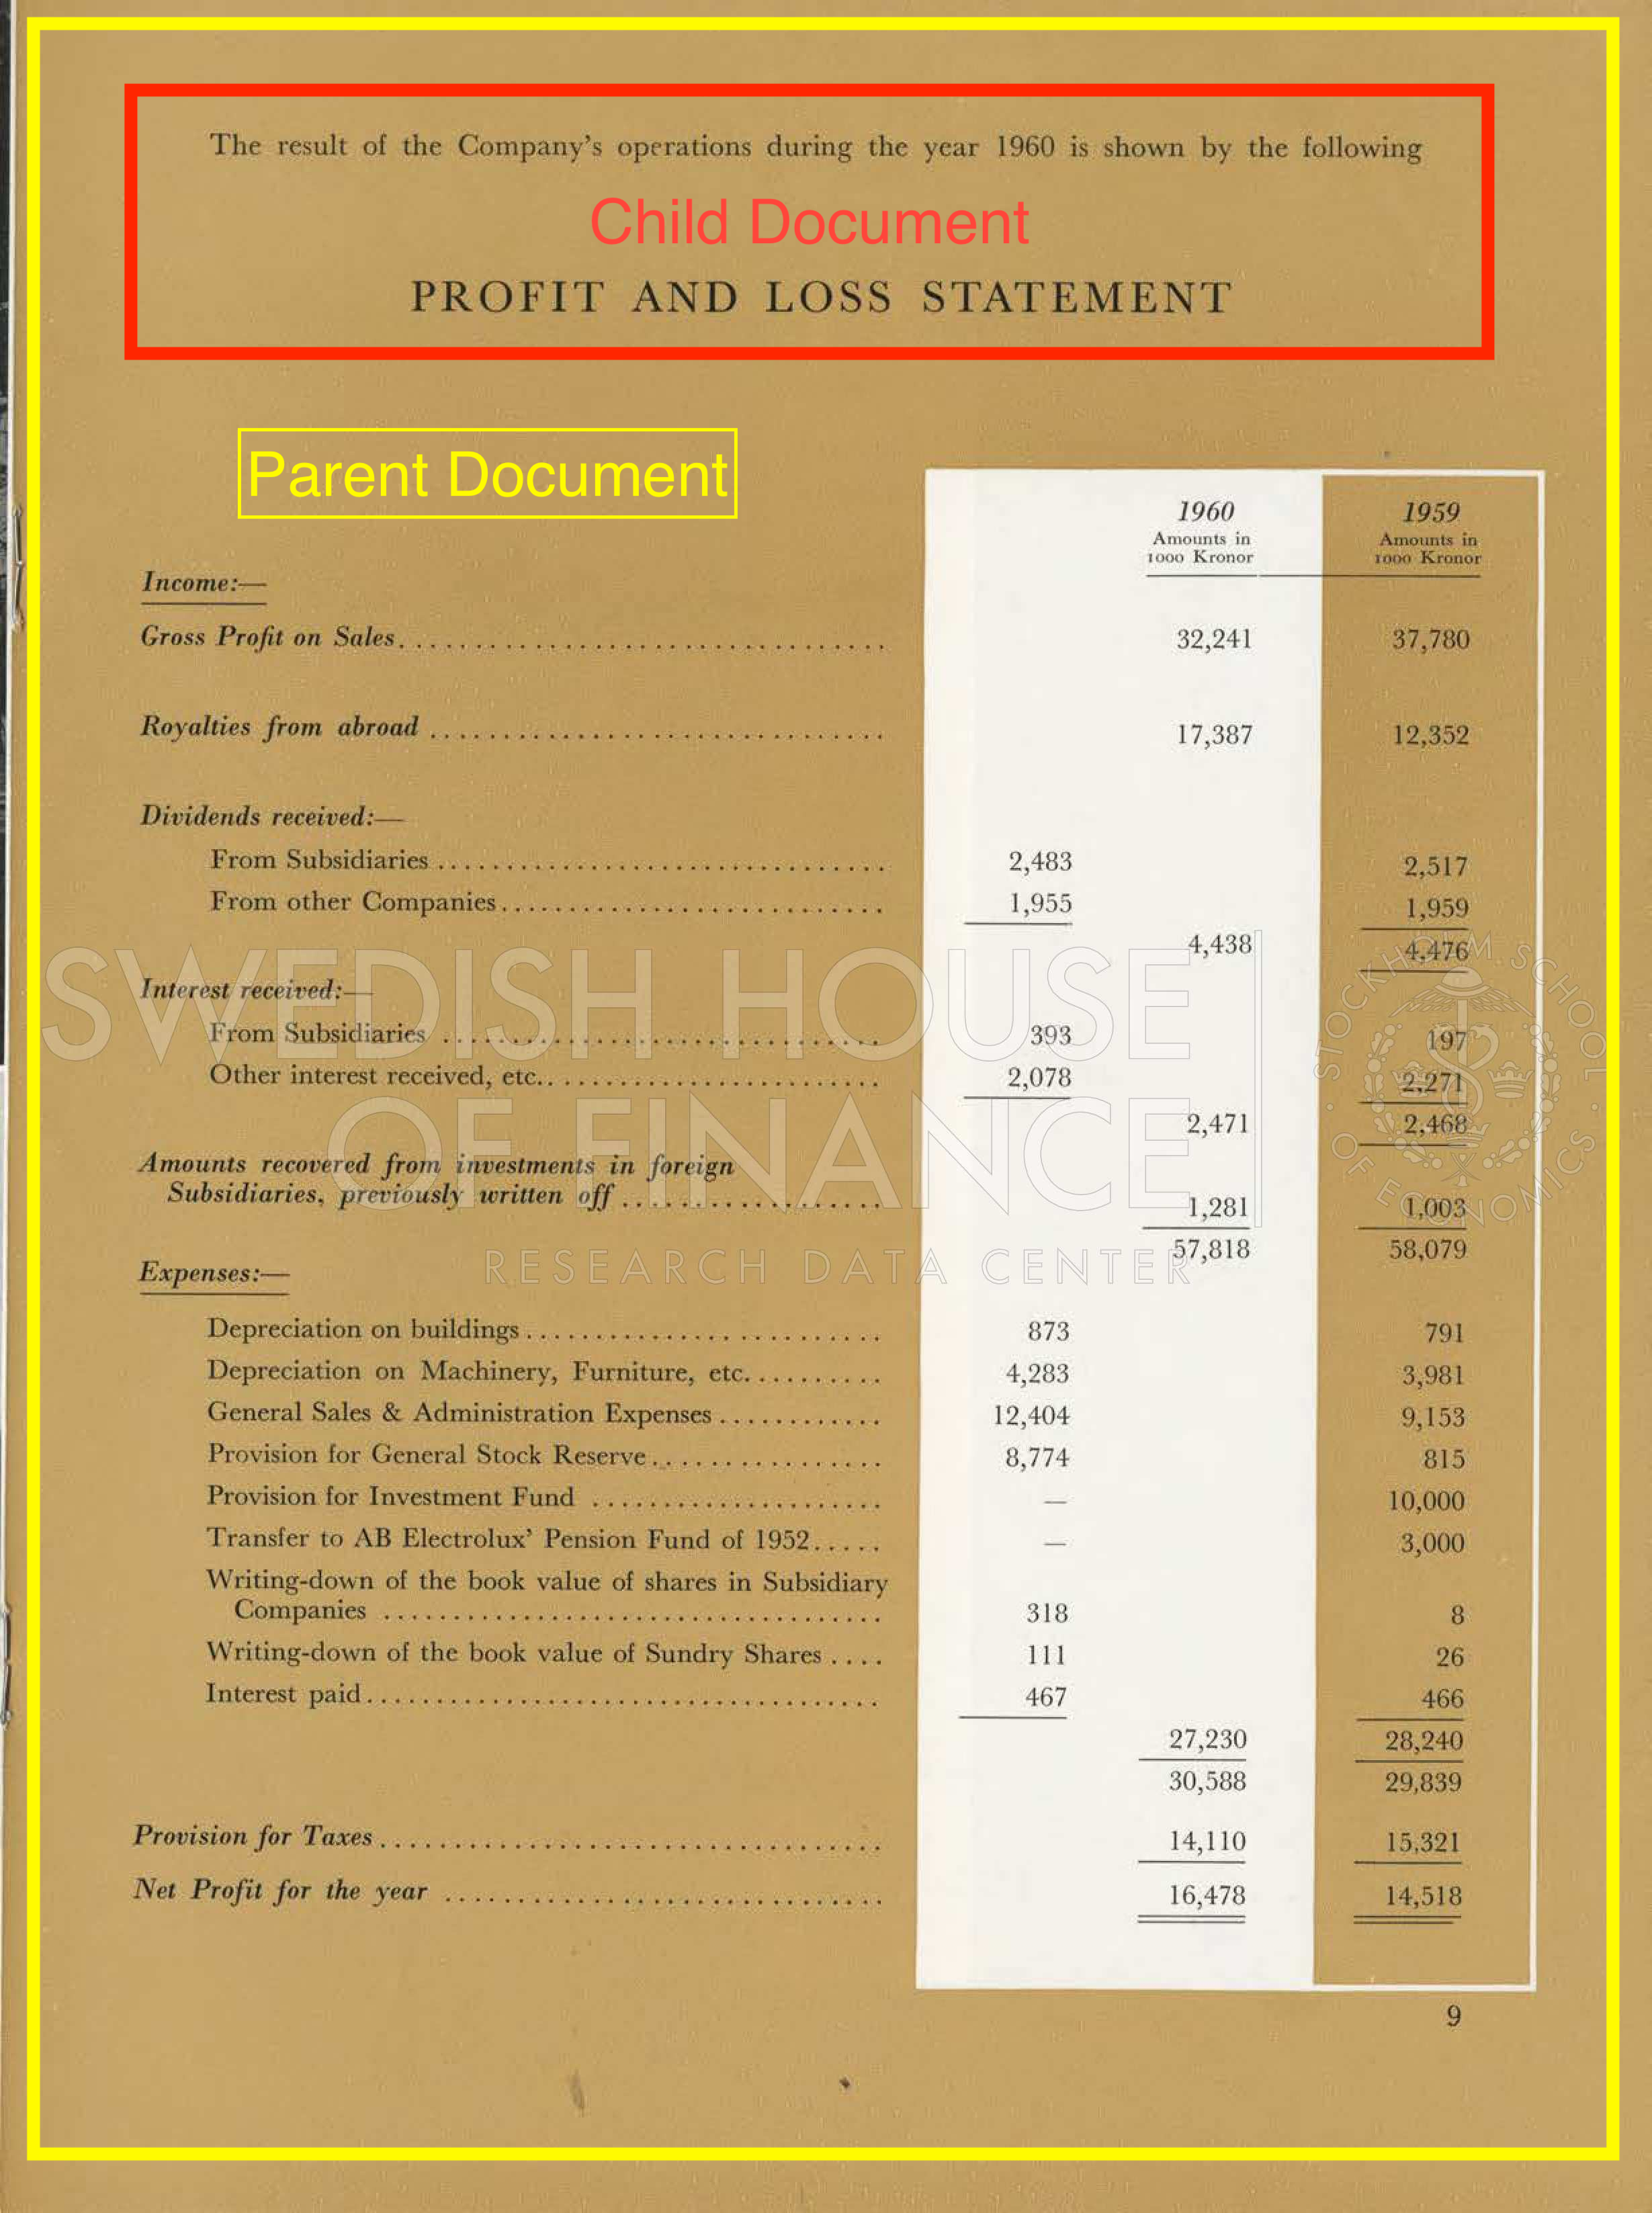
\includegraphics[width=1\textwidth,height=\textheight]{assets/Electrolux_1960_page_13.png}

\hypertarget{pass-the-page-to-gpt-4-vision-with-schema}{%
\subsection{Pass the page to GPT-4 Vision with
Schema}\label{pass-the-page-to-gpt-4-vision-with-schema}}

\begin{Shaded}
\begin{Highlighting}[]
\NormalTok{schema }\OperatorTok{=}\NormalTok{ [}
\NormalTok{        \{}
            \StringTok{"key"}\NormalTok{: }\StringTok{"year"}\NormalTok{,}
            \StringTok{"description"}\NormalTok{: }\StringTok{"The year for which the financial statement is being reported."}
\NormalTok{        \},}
\NormalTok{        \{}
            \StringTok{"key"}\NormalTok{: }\StringTok{"taxes"}\NormalTok{,}
            \StringTok{"description"}\NormalTok{: }\StringTok{"Total taxes paid by the company, also called \textquotesingle{}skatt\textquotesingle{} in Swedish"}
\NormalTok{        \},}
\NormalTok{        \{}
            \StringTok{"key"}\NormalTok{: }\StringTok{"net\_profit"}\NormalTok{,}
            \StringTok{"description"}\NormalTok{: }\StringTok{"Net profit earned by the company for the year, also called \textquotesingle{}Nettovinst för året\textquotesingle{} in Swedish"}
\NormalTok{        \}}
\NormalTok{]}

\NormalTok{payload }\OperatorTok{=}\NormalTok{ \{}
    \StringTok{"model"}\NormalTok{: }\StringTok{"gpt{-}4{-}vision{-}preview"}\NormalTok{,}
    \StringTok{"messages"}\NormalTok{: [}
\NormalTok{    \{}
        \StringTok{"role"}\NormalTok{: }\StringTok{"user"}\NormalTok{,}
        \StringTok{"content"}\NormalTok{: [}
\NormalTok{        \{}\StringTok{"type"}\NormalTok{: }\StringTok{"text"}\NormalTok{, }\StringTok{"text"}\NormalTok{: prompt\},}
\NormalTok{        \{}
            \StringTok{"type"}\NormalTok{: }\StringTok{"image\_url"}\NormalTok{,}
            \StringTok{"image\_url"}\NormalTok{: \{}
            \StringTok{"url"}\NormalTok{: }\SpecialStringTok{f"data:image/jpeg;base64,}\SpecialCharTok{\{}\NormalTok{base64\_image}\SpecialCharTok{\}}\SpecialStringTok{"}
\NormalTok{            \}}
\NormalTok{        \}}
\NormalTok{        ]}
\NormalTok{    \}}
\NormalTok{    ],}
    \StringTok{"max\_tokens"}\NormalTok{: }\DecValTok{1000}
\NormalTok{\}}
\end{Highlighting}
\end{Shaded}

\hypertarget{system-output}{%
\subsection{System output}\label{system-output}}

\begin{figure}

{\centering 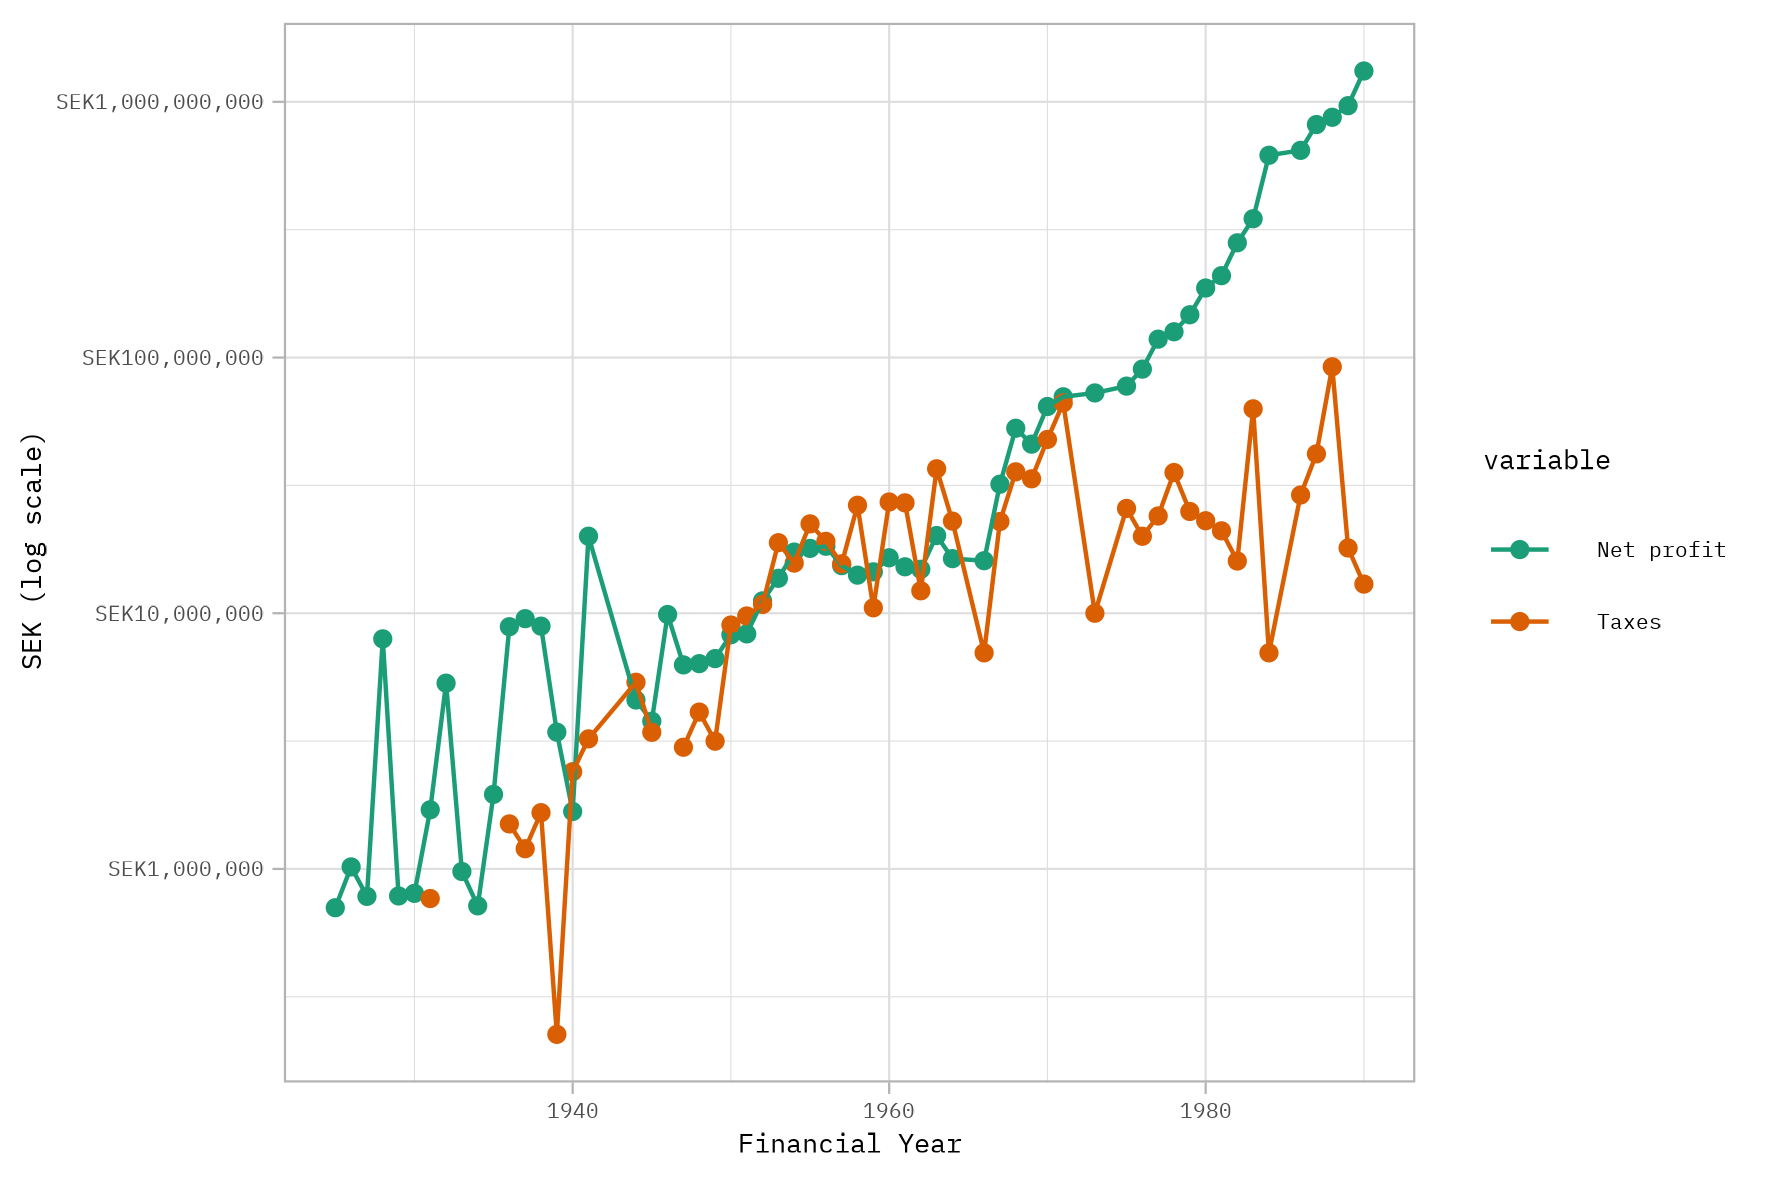
\includegraphics{assets/figures.png}

}

\caption{Electrolux Net Profit and Taxes}

\end{figure}

\hypertarget{why-does-this-work-well-what-are-the-limitations}{%
\subsection{Why does this work well? What are the
limitations?}\label{why-does-this-work-well-what-are-the-limitations}}

\textbf{Advantages}

\textbf{Skip step structuring with OCR}

\begin{itemize}
\tightlist
\item
  This is a difficult task
\item
  `Small' errors can lead to big problems
\item
  E.G 1,00 vs 1.00 or leading zeros
\end{itemize}

\textbf{`Read' the document like a research assistant}

\begin{itemize}
\tightlist
\item
  `Understand' the context of the tables
\end{itemize}

\textbf{Fast and cheap}

\begin{itemize}
\tightlist
\item
  2 mins processing time to get the result for 75 years of reports
\item
  After you've built the pipeline, switching to another company is easy
\end{itemize}

\textbf{Limitations}

\begin{itemize}
\tightlist
\item
  Requires clever schema design to get the data you want
\item
  Requires time to manually check outlier results
\item
  Works best with small tables
\item
  Not easily reproducible by others (though neither are research
  assistants)
\end{itemize}

\hypertarget{sec-conclusion}{%
\section{Conclusion}\label{sec-conclusion}}

Code available on my GitHub

I promise to answer any open issues!

\begin{figure}

{\centering 
\includegraphics{assets/qr-code.png}

}

\caption{\href{https://github.com/j-jayes/swedish-company-reports-data-extraction}{GitHub
Repo}}

\end{figure}



\end{document}
